\documentclass[a4paper]{article}

\def\npart {III}
\def\nterm {Lent}
\def\nyear {2018}
\def\nlecturer {S.\ Svaldi}
\def\ncourse {Positivity in Algebraic Geometry}

% Imports
\ifx \nextra \undefined
  \usepackage[pdftex,
    hidelinks,
    pdfauthor={Dexter Chua},
    pdfsubject={Cambridge Maths Notes: Part \npart\ - \ncourse},
    pdftitle={Part \npart\ - \ncourse},
  pdfkeywords={Cambridge Mathematics Maths Math \npart\ \nterm\ \nyear\ \ncourse}]{hyperref}
  \title{Part \npart\ - \ncourse}
\else
  \usepackage[pdftex,
    hidelinks,
    pdfauthor={Dexter Chua},
    pdfsubject={Cambridge Maths Notes: Part \npart\ - \ncourse\ (\nextra)},
    pdftitle={Part \npart\ - \ncourse\ (\nextra)},
  pdfkeywords={Cambridge Mathematics Maths Math \npart\ \nterm\ \nyear\ \ncourse\ \nextra}]{hyperref}

  \title{Part \npart\ - \ncourse \\ {\Large \nextra}}
\fi

\author{Lectured by \nlecturer \\\small Notes taken by Dexter Chua}
\date{\nterm\ \nyear}

\usepackage{alltt}
\usepackage{amsfonts}
\usepackage{amsmath}
\usepackage{amssymb}
\usepackage{amsthm}
\usepackage{booktabs}
\usepackage{caption}
\usepackage{enumitem}
\usepackage{fancyhdr}
\usepackage{graphicx}
\usepackage{mathtools}
\usepackage{microtype}
\usepackage{multirow}
\usepackage{pdflscape}
\usepackage{pgfplots}
\usepackage{siunitx}
\usepackage{tabularx}
\usepackage{tikz}
\usepackage{tkz-euclide}
\usepackage[normalem]{ulem}
\usepackage[all]{xy}

\pgfplotsset{compat=1.12}

\pagestyle{fancyplain}
\lhead{\emph{\nouppercase{\leftmark}}}
\ifx \nextra \undefined
  \rhead{
    \ifnum\thepage=1
    \else
      \npart\ \ncourse
    \fi}
\else
  \rhead{
    \ifnum\thepage=1
    \else
      \npart\ \ncourse\ (\nextra)
    \fi}
\fi
\usetikzlibrary{arrows}
\usetikzlibrary{decorations.markings}
\usetikzlibrary{decorations.pathmorphing}
\usetikzlibrary{positioning}
\usetikzlibrary{fadings}
\usetikzlibrary{intersections}
\usetikzlibrary{cd}

\newcommand*{\Cdot}{\raisebox{-0.25ex}{\scalebox{1.5}{$\cdot$}}}
\newcommand {\pd}[2][ ]{
  \ifx #1 { }
    \frac{\partial}{\partial #2}
  \else
    \frac{\partial^{#1}}{\partial #2^{#1}}
  \fi
}

% Theorems
\theoremstyle{definition}
\newtheorem*{aim}{Aim}
\newtheorem*{axiom}{Axiom}
\newtheorem*{claim}{Claim}
\newtheorem*{cor}{Corollary}
\newtheorem*{defi}{Definition}
\newtheorem*{eg}{Example}
\newtheorem*{fact}{Fact}
\newtheorem*{law}{Law}
\newtheorem*{lemma}{Lemma}
\newtheorem*{notation}{Notation}
\newtheorem*{prop}{Proposition}
\newtheorem*{thm}{Theorem}

\renewcommand{\labelitemi}{--}
\renewcommand{\labelitemii}{$\circ$}
\renewcommand{\labelenumi}{(\roman{*})}

\let\stdsection\section
\renewcommand\section{\newpage\stdsection}

% Strike through
\def\st{\bgroup \ULdepth=-.55ex \ULset}

% Maths symbols
\newcommand{\bra}{\langle}
\newcommand{\ket}{\rangle}

\newcommand{\N}{\mathbb{N}}
\newcommand{\Z}{\mathbb{Z}}
\newcommand{\Q}{\mathbb{Q}}
\renewcommand{\H}{\mathbb{H}}
\newcommand{\R}{\mathbb{R}}
\newcommand{\C}{\mathbb{C}}
\newcommand{\Prob}{\mathbb{P}}
\renewcommand{\P}{\mathbb{P}}
\newcommand{\E}{\mathbb{E}}
\newcommand{\F}{\mathbb{F}}
\newcommand{\cU}{\mathcal{U}}
\newcommand{\RP}{\mathbb{RP}}
\newcommand{\CP}{\mathbb{CP}}

\newcommand{\ph}{\,\cdot\,}

\DeclareMathOperator{\sech}{sech}
\DeclareMathOperator{\cosech}{cosech}
\DeclareMathOperator{\cosec}{cosec}

\DeclareMathOperator{\covol}{covol}
\DeclareMathOperator{\vol}{vol}

\let\Im\relax
\let\Re\relax
\DeclareMathOperator{\Im}{Im}
\DeclareMathOperator{\Re}{Re}
\DeclareMathOperator{\im}{im}
\DeclareMathOperator{\image}{image}
\DeclareMathOperator{\Ann}{Ann}

\DeclareMathOperator*{\res}{res}
\DeclareMathOperator{\Res}{Res}
\DeclareMathOperator{\Ind}{Ind}

\DeclareMathOperator{\tr}{tr}
\DeclareMathOperator{\diag}{diag}
\DeclareMathOperator{\rank}{rank}
\DeclareMathOperator{\card}{card}
\DeclareMathOperator{\spn}{span}
\DeclareMathOperator{\adj}{adj}

\DeclareMathOperator{\erf}{erf}
\DeclareMathOperator{\erfc}{erfc}

\DeclareMathOperator{\ord}{ord}
\DeclareMathOperator{\Sym}{Sym}

\DeclareMathOperator{\sgn}{sgn}
\DeclareMathOperator{\orb}{orb}
\DeclareMathOperator{\stab}{stab}
\DeclareMathOperator{\ccl}{ccl}

\DeclareMathOperator{\lcm}{lcm}
\DeclareMathOperator{\hcf}{hcf}

\DeclareMathOperator{\Int}{Int}
\DeclareMathOperator{\id}{id}

\DeclareMathOperator{\betaD}{beta}
\DeclareMathOperator{\gammaD}{gamma}
\DeclareMathOperator{\Poisson}{Poisson}
\DeclareMathOperator{\binomial}{binomial}
\DeclareMathOperator{\multinomial}{multinomial}
\DeclareMathOperator{\Bernoulli}{Bernoulli}
\DeclareMathOperator{\like}{like}

\DeclareMathOperator{\var}{var}
\DeclareMathOperator{\cov}{cov}
\DeclareMathOperator{\bias}{bias}
\DeclareMathOperator{\mse}{mse}
\DeclareMathOperator{\corr}{corr}

\DeclareMathOperator{\otp}{otp}
\DeclareMathOperator{\dom}{dom}

\DeclareMathOperator{\Root}{Root}
\DeclareMathOperator{\supp}{supp}
\DeclareMathOperator{\rel}{rel}
\DeclareMathOperator{\Hom}{Hom}
\DeclareMathOperator{\Aut}{Aut}
\DeclareMathOperator{\Gal}{Gal}
\DeclareMathOperator{\Mat}{Mat}
\DeclareMathOperator{\End}{End}
\DeclareMathOperator{\Char}{char}
\DeclareMathOperator{\ev}{ev}
\DeclareMathOperator{\St}{St}
\DeclareMathOperator{\Lk}{Lk}
\DeclareMathOperator{\disc}{disc}
\DeclareMathOperator{\Isom}{Isom}
\DeclareMathOperator{\length}{length}
\DeclareMathOperator{\energy}{energy}
\DeclareMathOperator{\area}{area}
\DeclareMathOperator{\Syl}{Syl}
\DeclareMathOperator{\cl}{cl}
\DeclareMathOperator{\fix}{fix}

\newcommand{\GL}{\mathrm{GL}}
\newcommand{\SL}{\mathrm{SL}}
\newcommand{\PGL}{\mathrm{PGL}}
\newcommand{\PSL}{\mathrm{PSL}}
\newcommand{\PSU}{\mathrm{PSU}}
\newcommand{\Or}{\mathrm{O}}
\newcommand{\SO}{\mathrm{SO}}
\newcommand{\U}{\mathrm{U}}
\newcommand{\SU}{\mathrm{SU}}

\renewcommand{\d}{\mathrm{d}}
\newcommand{\D}{\mathrm{D}}

\tikzset{->/.style = {decoration={markings,
                                  mark=at position 1 with {\arrow[scale=2]{latex'}}},
                      postaction={decorate}}}
\tikzset{<-/.style = {decoration={markings,
                                  mark=at position 0 with {\arrowreversed[scale=2]{latex'}}},
                      postaction={decorate}}}
\tikzset{<->/.style = {decoration={markings,
                                   mark=at position 0 with {\arrowreversed[scale=2]{latex'}},
                                   mark=at position 1 with {\arrow[scale=2]{latex'}}},
                       postaction={decorate}}}
\tikzset{->-/.style = {decoration={markings,
                                   mark=at position #1 with {\arrow[scale=2]{latex'}}},
                       postaction={decorate}}}
\tikzset{-<-/.style = {decoration={markings,
                                   mark=at position #1 with {\arrowreversed[scale=2]{latex'}}},
                       postaction={decorate}}}

\tikzset{circ/.style = {fill, circle, inner sep = 0, minimum size = 3}}
\tikzset{mstate/.style={circle, draw, blue, text=black, minimum width=0.7cm}}

\definecolor{mblue}{rgb}{0.2, 0.3, 0.8}
\definecolor{morange}{rgb}{1, 0.5, 0}
\definecolor{mgreen}{rgb}{0.1, 0.4, 0.2}
\definecolor{mred}{rgb}{0.5, 0, 0}

\def\drawcirculararc(#1,#2)(#3,#4)(#5,#6){%
    \pgfmathsetmacro\cA{(#1*#1+#2*#2-#3*#3-#4*#4)/2}%
    \pgfmathsetmacro\cB{(#1*#1+#2*#2-#5*#5-#6*#6)/2}%
    \pgfmathsetmacro\cy{(\cB*(#1-#3)-\cA*(#1-#5))/%
                        ((#2-#6)*(#1-#3)-(#2-#4)*(#1-#5))}%
    \pgfmathsetmacro\cx{(\cA-\cy*(#2-#4))/(#1-#3)}%
    \pgfmathsetmacro\cr{sqrt((#1-\cx)*(#1-\cx)+(#2-\cy)*(#2-\cy))}%
    \pgfmathsetmacro\cA{atan2(#2-\cy,#1-\cx)}%
    \pgfmathsetmacro\cB{atan2(#6-\cy,#5-\cx)}%
    \pgfmathparse{\cB<\cA}%
    \ifnum\pgfmathresult=1
        \pgfmathsetmacro\cB{\cB+360}%
    \fi
    \draw (#1,#2) arc (\cA:\cB:\cr);%
}
\newcommand\getCoord[3]{\newdimen{#1}\newdimen{#2}\pgfextractx{#1}{\pgfpointanchor{#3}{center}}\pgfextracty{#2}{\pgfpointanchor{#3}{center}}}

\def\Xint#1{\mathchoice
   {\XXint\displaystyle\textstyle{#1}}%
   {\XXint\textstyle\scriptstyle{#1}}%
   {\XXint\scriptstyle\scriptscriptstyle{#1}}%
   {\XXint\scriptscriptstyle\scriptscriptstyle{#1}}%
   \!\int}
\def\XXint#1#2#3{{\setbox0=\hbox{$#1{#2#3}{\int}$}
     \vcenter{\hbox{$#2#3$}}\kern-.5\wd0}}
\def\ddashint{\Xint=}
\def\dashint{\Xint-}


\newcommand\A{\mathbb{A}}
\newcommand\val{\mathrm{val}}
\renewcommand\div{\mathrm{div}}
\newcommand\Cl{\mathrm{Cl}}
\newcommand\WDiv{\mathrm{WDiv}}
\newcommand\Div{\mathrm{Div}}
\newcommand\CaDiv{\mathrm{CaDiv}}
\newcommand\Pic{\mathrm{Pic}}
\newcommand\Num{\mathrm{Num}}
\newcommand\Amp{\mathrm{Amp}}
\newcommand\Nef{\mathrm{Nef}}
\newcommand\NS{\mathrm{NS}}
\newcommand\NE{\mathrm{NE}}
\newcommand\Bl{\mathrm{Bl}}
\DeclareMathOperator\red{red}
\DeclareMathOperator\Proj{Proj}

\begin{document}
\maketitle
{\small
\setlength{\parindent}{0em}
\setlength{\parskip}{1em}
This class aims at giving an introduction to the theory of divisors, linear systems and their positivity properties on projective algebraic varieties.

The first part of the class will be dedicated to introducing the basic notions and results regarding these objects and special attention will be devoted to discussing examples in the case of curves and surfaces.

In the second part, the course will cover classical results from the theory of divisors and linear systems and their applications to the study of the geometry of algebraic varieties.

If time allows and based on the interests of the participants, there are a number of more advanced topics that could possibly be covered: Reider's Theorem for surfaces, geometry of linear systems on higher dimensional varieties, multiplier ideal sheaves and invariance of plurigenera, higher dimensional birational geometry.

\subsubsection*{Pre-requisites}
The minimum requirement for those students wishing to enroll in this class is their knowledge of basic concepts from the Algebraic Geometry Part 3 course, i.e.\ roughly Chapters 2 and 3 of Hartshorne's Algebraic Geometry.

Familiarity with the basic concepts of the geometry of algebraic varieties of dimension 1 and 2 --- e.g.\ as covered in the preliminary sections of Chapters 4 and 5 of Hartshorne's Algebraic Geometry --- would be useful but will not be assumed --- besides what was already covered in the Michaelmas lectures.

Students should have also some familiarity with concepts covered in the Algebraic Topology Part 3 course such as cohomology, duality and characteristic classes.
}
\tableofcontents

%\section{Introduction}
%Fix a field $K$. The first problem we want to look at is the following:
%\begin{problem}
%  Classify all finitely-generated field extension $L/K$.
%\end{problem}
%A closely related problem is
%\begin{problem}
%  Classify all towers of field extensions $L/M/K$.
%\end{problem}
%In general, we don't want to consider finite extensions --- this falls within the scope of Galois theory instead.
%
%In general, given a finite extension $L/K$, we can factorize it into a tower $L/M/K$, where $M/K$ is purely transcendental, i.e.\ $M \cong K(x_1, \ldots, x_n)$ is a field of rational functions over $K$.
%
%A large class of examples comes from \term{function fields} of algebraic varieties, $K(X)$.
%\begin{eg}
%  Recall that if $X$ is affine, then $K(X)$ is the field of fractions of the ring of functions of $X$, i.e.\ $Q(K[X])$.
%\end{eg}
%
%\begin{question}
%  Are these all the examples of finitely-generated field extensions $L/K$?
%\end{question}
%
%
%\begin{lemma}
%  Let $\Char K = 0$. If $L/K$ is finitely-generated and not finite, then there exists an algebraic variety $X/K$ such that $K(X) \cong L$.
%\end{lemma}
%Note that the condition is satisfied in particular if $K$ is algebraically closed.
%
%\begin{proof}
%  We factor $L/M/K$, where $M/K$ is purely transcendental, say $M = K(x_1, \ldots, x_n) = K(\A^n)$. Since $\Char(K) = 0$, we can use the primitive element theorem to get that $L = M(\alpha)$ for some $\alpha \in L$. Then if $f$ is the minimal polynomial for $\alpha$, then
%  \[
%    L \cong Q(K[x_1, \ldots, x_n, x]/(f(x))).\qedhere
%  \]
%\end{proof}
%
%
%now suppose $\varphi: x \to y$ is a dominant birational map, % make birational
%i.e.\ $\overline{\varphi(X)} = Y$. Then this induces a map $\varphi^* : K(Y) \to K(X)$.
%
%Indeed, an element of $K(Y)$ is just a rational function $Y \to \A^1_K$, and pre-composing with $\varphi$ gives the desired function. The dominance ensures the composition is well-defined.
%
%Now if every embedding of field extensions arise this way, then we have reduced our problem to studying algebraic varieties over $K$ and their rational dominant maps. This is indeed the case.
%\begin{thm}
%  Let $K$ be a field with $\Char K = 0$. Then there is an equivalence of categories between
%  \[
%    \left\{ \parbox{4.8cm}{\centering algebraic varieties over $K$\\ rational dominant morphisms}\right\} \longleftrightarrow \left\{\parbox{5.3cm}{\centering infinite f.g.\ field extensions over $K$\\field embeddings}\right\}
%  \]
%\end{thm}
%
%\begin{proof}
%  We define a functor from the left category to the right by sending a variety $X$ to the field of rational functions on $X$, $K(X)$, and morphisms are as above. We have already seen that this is essentially surjective. To show it is fully faithful, suppose $X, Y$ are algebraic varieties over $K$, and $\psi: K(Y) \hookrightarrow K(X)$. We want to show that $\psi = \varphi^*$ for some rational dominant map $X \to Y$.
%
%  We can assume that $X$ and $Y$ are affine, since every variety is birationally equivalent to any Zariski open subset. Then $K(X) = Q(K[X])$ and $K(Y) = Q(K[Y])$. So in particular, we have an embedding $K[Y] \hookrightarrow K(X)$. Since $K[Y]$ is finitely-generated, we can produce a factorization
%  \[
%    \begin{tikzcd}
%      K[Y] \ar[r, hook] \ar[dr, hook] & K(X) \\
%      & K[X]_{s_1, \ldots, s_n} \ar[u, hook]
%    \end{tikzcd}
%  \]
%  for some $s_1, \ldots, s_n$. But then $K[X]_{s_1, \ldots, s_n} = K[U]$ for some open $U \subseteq X$. Then the map $K[Y] \to K[U]$ determines a map $U \to Y$, hence a rational map $X \to Y$. The injectivity of the map $K[Y] \to K[U]$ corresponds to the fact that the induced map $U \to Y$ is dominant. So we are done.
%\end{proof}
%
\section{Divisors}
\subsection{Projective embeddings}
Our results here will be stated for rather general schemes, since we can, but at the end, we are only interested in concrete algebraic varieties.

We are interested in the following problem --- given a scheme $X$, can we embed it in projective space? The first observation that $\P^n$ comes with a very special line bundle $\mathcal{O}(1)$, and every embedding $X \hookrightarrow \P^n$ gives pulls back to a corresponding sheaf $\mathcal{L}$ on $X$.

The key property of $\mathcal{O}(1)$ is that it has \emph{global} sections $x_0, \ldots, x_n$ which generate $\mathcal{O}(1)$ as an $\mathcal{O}_X$-module.

\begin{defi}[Generating section]\index{generating section}
  Let $X$ be a scheme, and $\mathcal{F}$ a sheaf of $\mathcal{O}_X$-modules. Let $s_0, \ldots, s_n \in H^0(X, \mathcal{F})$ be sections. We say the sections \emph{generate} $\mathcal{F}$ if the natural map
  \[
    \bigoplus_{i = 0}^{n + 1} \mathcal{O}_X \to \mathcal{F}
  \]
  induced by the $s_i$ is a surjective map of $\mathcal{O}_X$-modules.
\end{defi}

The generating sections are preserved under pullbacks. So if $X$ is embedded into $\P^n$, then it should have a corresponding line bundle generated by $n + 1$ global sections. More generally, if there is any map to $\P^n$ at all, we can pull back a corresponding bundle. Indeed, we have the following theorem:
\begin{thm}
  Let $A$ be any ring, and $X$ a scheme over $A$.
  \begin{enumerate}
    \item If $\varphi: X \to \P^n$ is a morphism over $A$, then $\varphi^* \mathcal{O}_{\P^n}(1)$ is an invertible sheaf on $X$, generated by the sections $\varphi^* x_0, \ldots, \varphi^* x_n \in H^0(X, \varphi^* \mathcal{O}_{\P^n}(1))$.
    \item If $\mathcal{L}$ is an invertible sheaf on $X$, and if $s_0, \ldots, s_n \in H^0(X, \mathcal{L})$ which generate $\mathcal{L}$, then there exists a unique morphism $\varphi: X \to \P^n$ such that $\varphi^* \mathcal{O}(1) \cong \mathcal{L}$ and $\varphi^* x_i = s_i$.
  \end{enumerate}
\end{thm}

This theorem highlights the importance of studying line bundles and their sections, and in some sense, understanding these is the whole focus of the course.

\begin{proof}\leavevmode
  \begin{enumerate}
    \item The pullback of an invertible sheaf is an invertible, and the pullbacks of $x_0, \ldots, x_n$ generate $\varphi^* \mathcal{O}_{\P^n}(1)$.

    \item In short, we map $x \in X$ to $[s_0(x): \cdots : s_n(x)] \in \P^n$.

      In more detail, define
      \[
        X_{s_i} = \{p \in X: s_i \not\in \mathfrak{m}_p \mathcal{L}_p\}.
      \]
      This is a Zariski open set, and $s_i$ is invertible on $X_{s_i}$. Thus there is a dual section $s_i^\vee \in \mathcal{L}^{\vee}$ such that $s_i \otimes s_i^\vee \in \mathcal{L} \otimes \mathcal{L}^\vee \cong \mathcal{O}_X$ is equal to $1$. Define the map $X_{s_i} \to \A^n$ by the map
      \begin{align*}
        K[\A^n] &\to H^0(X_{s_i}, \mathcal{O}_{s_i})\\
        y_i &\mapsto s_j \otimes s_i^\vee.
      \end{align*}
      Since the $s_i$ generate, they cannot simultaneously vanish on a point. So $X = \bigcup X_{s_i}$. Identifying $\A^n$ as the chart of $\P^n$ where $x_i \not= 0$, this defines the desired map $X \to \P^n$.\qedhere
  \end{enumerate}
\end{proof}

The theorem tells us we get a map from $X$ to $\P^n$. However, it says nothing about how nice these maps are. In particular, it says nothing about whether or not we get an embedding.

\begin{defi}[Very ample sheaf]\index{very ample sheaf}\index{sheaf!very ample}
  Let $X$ be an algebraic variety over $K$, and $\mathcal{L}$ be an invertible sheaf. We say that $\mathcal{L}$ is very ample if there is a closed immersion $\varphi: X \to \P^n$ such that $\varphi^* \mathcal{O}_{\P^n}(1) \cong \mathcal{L}$.
\end{defi}
It would be convenient if we had a good way of identifying when $\mathcal{L}$ is very ample. In this section, we will prove some formal criteria for very ampleness, which are convenient for proving things but not very convenient for actually checking if a line bundle is very ample. In specific cases, such as for curves, we can obtain some rather more concrete and usable criterion.

So how can we understand when a map $X \hookrightarrow \P^n$ is an embedding? If it were an embedding, then it in particular is injective. So given any two points in $X$, there is a hyperplane in $\P^n$ that passes through one but not the other. But being an embedding means something more. We want the differential of the map to be injective as well. This boils down to the following conditions:

\begin{prop}
  Let $K = \bar{K}$, and $X$ a projective variety over $K$. Let $\mathcal{L}$ be an invertible sheaf on $X$, and $s_0, \ldots, s_n \in H^0(X, \mathcal{L})$ generating sections. Write $V = \bra s_0, \ldots, s_n\ket$ for the linear span. Then the associated map $\varphi: X \to \P^n$ is a closed embedding iff
  \begin{enumerate}
    \item For every distinct closed points $p \not= q \in X$, there exists $s_{p, q} \in V$ such that $s_{p, q} \in \mathfrak{m}_p \mathcal{L}_p$ but $s_{p, q} \not \in \mathfrak{m}_q \mathcal{L}_q$.
    \item For every closed point $p \in X$, the set $\{s \in V \mid s \in \mathfrak{m}_p \mathcal{L}_p\}$ spans the vector space $\mathfrak{m}_p \mathcal{L}_p /\mathfrak{m}^2_p \mathcal{L}_p$.
  \end{enumerate}
\end{prop}

\begin{defi}[Separate points and tangent vectors]
  With the hypothesis of the proposition, we say that
  \begin{itemize}
    \item elements of $V$ \term{separate points} if $V$ satisfies (i).
    \item elements of $V$ \term{separate tangent vectors} if $V$ satisfies (ii).
  \end{itemize}
\end{defi}

\begin{proof}\leavevmode
  \begin{itemize}
    \item[$(\Rightarrow)$] Suppose $\phi$ is a closed immersion. Then it is injective on points. So suppose $p \not= q$ are (closed) points. Then there is some hyperplane $H_{p, q}$ in $\P^n$ passing through $p$ but not $q$. The hyperplane $H_{p, q}$ is the vanishing locus of a global section of $\mathcal{O}(1)$. Let $s_{p, q} \in V \subseteq H^0(X, \mathcal{L})$ be the pullback of this section. Then $s_{p, q} \in \mathfrak{m}_p \mathcal{L}_p$ and $s_{p, q} \not \in \mathfrak{m}_q \mathcal{L}_q$. So (i) is satisfied.

      To see (ii), we restrict to the affine patch containing $p$, and $X$ is a closed subvariety of $\A^n$. The result is then clear since $\mathfrak{m}_p\mathcal{L}_p/\mathfrak{m}_p^2\mathcal{L}_p$ is exactly the span of $s_0, \ldots, s_n$. We used $K = \bar{K}$ to know what the closed points of $\P^n$ look like.

    \item[$(\Leftarrow)$] We first show that $\varphi$ is injective on closed points. For any $p \not= q \in X$, write the given $s_{p, q}$ as
      \[
        s_{p, q} = \sum \lambda_i s_i = \sum \lambda_i \varphi^* x_i = \varphi^* \sum \lambda_i x_i
      \]
      for some $\lambda_i \in K$. So we can take $H_{p, q}$ to be given by the vanishing set of $\sum \lambda_i x_i$, and so it is injective on closed point. It follows that it is also injective on schematic points. Since $X$ is proper, so is $\varphi$, and in particular $\varphi$ is a homeomorphism onto the image.

      To show that $\varphi$ is in fact a closed immersion, we need to show that $\mathcal{O}_{\P^n} \to \varphi_* \mathcal{O}_X$ is surjective. As before, it is enough to prove that it holds at the level of stalks over closed points. To show this, we observe that $\mathcal{L}_p$ is trivial, so $\mathfrak{m}_p\mathcal{L}_p/\mathfrak{m}^2_p\mathcal{L}_p \cong \mathfrak{m}_p/\mathfrak{m}^2_p$ (unnaturally). We then apply the following lemma:
      \begin{lemma}
        Let $f: A \to B$ be a local morphism of local rings such that
        \begin{itemize}
          \item $A/\mathfrak{m}_A \to B/\mathfrak{m}_B$ is an isomorphism;
          \item $\mathfrak{m}_A \to \mathfrak{m}_B/\mathfrak{m}_B^2$ is surjective; and
          \item $B$ is a finitely-generated $A$-module.
        \end{itemize}
        Then $f$ is surjective.\fakeqed
      \end{lemma}
      To check the first condition, note that we have
      \[
        \frac{\mathcal{O}_{p, \P^n}}{\mathfrak{m}_{p, \P^n}} \cong \frac{\mathcal{O}_{p, X}}{\mathfrak{m}_{p, X}} \cong K.
      \]
      Now since $\mathfrak{m}_{p, \P^n}$ is generated by $x_0, \ldots, x_n$, the second condition is the same as saying
      \[
        \mathfrak{m}_{p, \P^n} \to \frac{\mathfrak{m}_{p, X}}{\mathfrak{m}_{p, X}^2}
      \]
      is surjective. The last part is immediate.\qedhere
  \end{itemize}
\end{proof}
Unsurprisingly, this is not a very pleasant hypothesis to check, since it requires us to really understand the structure of $V$. In general, given an invertible sheaf $\mathcal{L}$, it is unlikely that we can concretely understand the space of sections. It would be nice if there is some simpler criterion to check if sheaves are ample.

One convenient place to start is the following theorem of Serre:
\begin{thm}[Serre]
  Let $X$ be a projective scheme over a Noetherian ring $A$, $\mathcal{L}$ be a very ample invertible sheaf, and $\mathcal{F}$ a coherent $\mathcal{O}_X$-module. Then there exists a positive integer $n_0 = n_0(\mathcal{F}, \mathcal{L})$ such that for all $n \geq n_0$, the twist $\mathcal{F} \otimes \mathcal{L}^n$ is generated by global sections.\fakeqed
\end{thm}
The proof of this is straightforward and will be omitted. The idea is that tensoring with $\mathcal{L}^n$ lets us clear denominators, and once we have cleared all the denominators of the (finitely many) generators of $\mathcal{F}$, the resulting sheaf $\mathcal{F} \otimes \mathcal{L}^n$ will be generated by global sections.

We can weaken the condition of very ampleness to only require the condition of this theorem to hold.
\begin{defi}[Ample sheaf]\index{ample sheaf}
  Let $X$ be a Noetherian scheme over $A$, and $\mathcal{L}$ an invertible sheaf over $X$. We say $\mathcal{L}$ is ample iff for any coherent $\mathcal{O}_X$-module $\mathcal{F}$, there is an $n_0$ such that for all $n \geq n_0$, the sheaf $\mathcal{F} \otimes \mathcal{L}^n$ is generated by global sections.
\end{defi}

While this seems like a rather weak condition, it is actually not too bad. First of all, by taking $\mathcal{F}$ to be $\mathcal{O}_X$, we can find some $\mathcal{L}^n$ that is generated by global sections. So at least it gives some map to $\P^n$. In fact, another theorem of Serre tells us this gives us an embedding.

\begin{thm}[Serre]
  Let $X$ be a scheme of finite type over a Noetherian ring $A$, and $\mathcal{L}$ an invertible sheaf on $X$. Then $\mathcal{L}$ is ample iff there exists $m > 0$ such that $\mathcal{L}^m$ is very ample.
\end{thm}

\begin{proof}\leavevmode
  \begin{itemize}
    \item[($\Leftarrow$)] Let $\mathcal{L}^m$ be very ample, and $\mathcal{F}$ a coherent sheaf. By Serre's theorem, there exists $n_0$ such that for all $j \geq j_0$, the sheafs
      \[
        \mathcal{F} \otimes \mathcal{L}^{mj}, (\mathcal{F} \otimes \mathcal{L}) \otimes \mathcal{L}^{mj}, \ldots, (\mathcal{F} \otimes \mathcal{L}^{m - 1}) \otimes \mathcal{L}^{mj}
      \]
      are all globally generated. So $\mathcal{F} \otimes \mathcal{L}^n$ is globally generated for $n \geq mj_0$.
    \item[($\Rightarrow$)] Suppose $\mathcal{L}$ is ample. Then $\mathcal{L}^m$ is globally generated for $m$ sufficiently large. We claim that there exists $t_1, \ldots, t_n \in H^0(X, \mathcal{L}^N)$ such that $\mathcal{L}|_{X_{t_i}}$ are all trivial (i.e.\ isomorphic to $\mathcal{O}_{X_{t_i}}$), and $X = \bigcup X_{t_i}$.

      By compactness, it suffices to show that for each $p \in X$, there is some $t \in H^0(X, \mathcal{L}^n)$ (for some $n$) such that $p \in X_{t_i}$ and $\mathcal{L}$ is trivial on $X_{t_i}$. First of all, since $\mathcal{L}$ is locally free by definition, we can find an open affine $U$ containing $p$ such that $\mathcal{L}|_U$ is trivial.

      Thus, it suffices to produce a section $t$ that vanishes on $Y = X - U$ but not at $p$. Then $p \in X_t \subseteq U$ and hence $\mathcal{L}$ is trivial on $X_t$. Vanishing on $Y$ is the same as belonging to the ideal sheaf $\mathcal{I}_Y$. Since $\mathcal{I}_Y$ is coherent, ampleness implies there is some large $n$ such that $\mathcal{I}_Y \otimes \mathcal{L}^n$ is generated by global sections. In particular, since $\mathcal{I}_Y \otimes \mathcal{L}^n$ doesn't vanish at $p$, we can find some $t \in \Gamma(X, \mathcal{I}_Y \otimes \mathcal{L}^N)$ such that $t \not \in \mathfrak{m}_p (\mathcal{I}_Y \otimes \mathcal{L}^n)_p$. Since $\mathcal{I}_Y$ is a subsheaf of $\mathcal{O}_X$, we can view $t$ as a section of $\mathcal{L}^n$, and this $t$ works.

      Now given the $X_{t_i}$, for each fixed $i$, we let $\{b_{ij}\}$ generate $\mathcal{O}_{X_{t_i}}$ as an $A$-algebra. Then for large $n$, $c_{ij} = t_i^n b_{ij}$ extends to a global section $c_{ij} \in \Gamma(X, \mathcal{L}^n)$ (by clearing denominators). We can pick an $n$ large enough to work for all $b_{ij}$. Then we use $\{t_i^n, c_{ij}\}$ as our generating sections to construct a morphism to $\P^N$, and let $\{x_i, x_{ij}\}$ be the corresponding coordinates. Observe that $\bigcup X_{t_i} = X$ implies the $t_i^n$ already generate $\mathcal{L}^n$. Now each $x_{t_i}$ gets mapped to $U_i \subseteq \P^N$, the vanishing set of $x_i$. The map $\mathcal{O}_{U_i} \to \varphi_* \mathcal{O}_{X_{t_i}}$ corresponds to the map
      \[
        A[y_i, y_{ij}] \to \mathcal{O}_{X_{t_i}},
      \]
      where $y_{ij}$ is mapped to $c_{ij}/t_i^n = b_{ij}$. So by assumption, this is surjective, and so we have a closed embedding.\qedhere
  \end{itemize}
\end{proof}

From this, we also see that
\begin{prop}
  Let $\mathcal{L}$ be a sheaf over $X$ (which is itself a projective variety over $K$). Then the following are equivalent:
  \begin{enumerate}
    \item $\mathcal{L}$ is ample.
    \item $\mathcal{L}^m$ is ample for all $m > 0$.
    \item $\mathcal{L}^m$ is ample for some $m > 0$.\fakeqed
  \end{enumerate}
\end{prop}

We will also frequently make use of the following theorem:
\begin{thm}[Serre]
  Let $X$ be a projective scheme over a Noetherian ring $A$, and $\mathcal{L}$ is very ample on $X$. Let $\mathcal{F}$ be a coherent sheaf. Then
  \begin{enumerate}
    \item For all $i \geq 0$ and $n \in \N$, $H^i(\mathcal{F} \otimes \mathcal{L}^n)$ is a finitely-generated $A$-module.
    \item There exists $n_0 \in \N$ such that for all $n \geq n_0$, $H^i(\mathcal{F} \otimes \mathcal{L}^n) = 0$ for all $i > 0$.\fakeqed
  \end{enumerate}
\end{thm}
The proof is exactly the same as the case of $\mathcal{O}(1)$ on $\P^n$.

As before, this theorem still holds for ample sheaves, and in fact characterizes them.
\begin{thm}
  Let $X$ be a proper scheme over a Noetherian ring $A$, and $\mathcal{L}$ an invertible sheaf. Then the following are equivalent:
  \begin{enumerate}
    \item $\mathcal{L}$ is ample.
    \item For all coherent $\mathcal{F}$ on $X$, there exists $n_0 \in \N$ such that for all $n \geq n_0$, we have $H^i(\mathcal{F} \otimes \mathcal{L}^n) = 0$.
  \end{enumerate}
\end{thm}

\begin{proof}
  Proving (i) $\Rightarrow$ (ii) is the same as the first part of the theorem last time.

  To prove (ii) $\Rightarrow$ (i), fix a point $x \in X$, and consider the sequence
  \[
    0 \to \mathfrak{m}_x \mathcal{F} \to \mathcal{F} \to \mathcal{F}_x \to 0.
  \]
  We twist by $\mathcal{L}^n$, where $n$ is sufficiently big, and take cohomology. Then we have a long exact sequence
  \[
    0 \to H^0(\mathfrak{m}_x \mathcal{F}(n)) \to H^0(\mathcal{F}(n)) \to H^0(\mathcal{F}_x(n)) \to H^1(\mathfrak{m}_x \mathcal{F}(n)) = 0.
  \]
  In particular, the map $H^0(\mathcal{F}(n)) \to H^0(\mathcal{F}_x(n))$ is surjective. This mean at $x$, $\mathcal{F}(n)$ is globally generated. Then by compactness, there is a single $n$ large enough such that $\mathcal{F}(n)$ is globally generated everywhere.
\end{proof}

\subsection{Weil divisors}
If $X$ is a sufficiently nice Noetherian scheme, $\mathcal{L}$ is a line bundle over $X$, and $s \in H^0(X, \mathcal{L})$, then the vanishing locus of $s$ is a codimension-$1$ subscheme. More generally, if $s$ is a rational section, then the zeroes and poles form codimension $1$ subschemes. Thus, to understand line bundles, a good place to start would be to understand these subschemes. We will see that for suitably nice schemes, we can recover $\mathcal{L}$ completely from this information.

For the theory to work out nicely, we need to assume the following technical condition:
\begin{defi}[Regular in codimension 1]\index{regular in codimension 1}
  Let $X$ be a Noetherian scheme. We say $X$ is \emph{regular in codimension 1} if every local ring $\mathcal{O}_x$ of dimension $1$ is regular.
\end{defi}
The key property of such schemes we will make use of is that if $Y \subseteq X$ is a codimension $1$ integral subscheme, then the local ring $\mathcal{O}_{X, Y}$ is a DVR. Then there is a valuation
\[
  \val_Y: \mathcal{O}_{X, Y} \to \Z,
\]
which tells us the order of vanishing/poles of our function along $Y$.

\begin{defi}[Weil divisor]\index{Weil divisor}
  Let $X$ be a Noetherian scheme, regular in codimension $1$. A \term{prime divisor} is a codimension $1$ integral subscheme of $X$. A \emph{Weil divisor} is a formal sum
  \[
    D = \sum a_i Y_i,
  \]
  where the $a_i \in \Z$ and $Y_i$ are prime divisors. We write $\WDiv(X)$ for the group of Weil divisors of $X$.

  For $K$ a field, a \term{Weil $K$-divisor} is the same where we allow $a_i \in K$.
\end{defi}

\begin{defi}[Effective divisor]\index{effective divisor}
  We say a Weil divisor is \emph{effective} if $a_i \geq 0$ for all $i$. We write $D \geq 0$.
\end{defi}

\begin{defi}[Principal divisor]\index{principal divisor}\index{$\mathrm{div}(f)$}
  If $f \in K(X)$, then we define the \emph{principal divisor}
  \[
    \div(f) = \sum_{Y} \val_Y(f) \cdot Y.
  \]
\end{defi}
One can show that $\val_Y(f)$ is non-zero for only finitely many $Y$'s, so this is a genuine divisor. To see this, there is always a Zariski open $U$ such that $f|_U$ is invertible, So $\val_Y(f) \not= 0$ implies $Y \subseteq X \setminus U$. Since $X$ is Noetherian, $X \setminus U$ can only contain finitely many codimension $1$ subscheme.

\begin{defi}[Support]\index{support}
  The \emph{support} of $D = \sum a_i Y_i$ is
  \[
    \supp(D) = \bigcup Y_i.
  \]
\end{defi}

Observe that $\div(fg) = \div(f) + \div(g)$. So the principal divisors form a subgroup of the Weil divisors.

\begin{defi}[Class group]\index{class group}
  The \emph{class group} of $X$, $\Cl(X)$, is the group of Weil divisors quotiented out by the principal divisors.

  We say Weil divisors $D, D'$ are \term{linearly equivalent} if $D - D'$ is principal, and we write $D \sim D'$.
\end{defi}

\begin{eg}
  Take $X = \A^1_K$, and $f = \frac{x^3}{x + 1} \in K(X)$. Then
  \[
    \div(f) = 3[0] - [-1].
  \]
\end{eg}

A useful result for the future is the following:
\begin{thm}[Hartog's lemma]\index{Hartog's lemma}
  Let $X$ be normal, and $f \in \mathcal{O}(X \setminus V)$ for some $V \geq 2$. Then $f \in \mathcal{O}_X$. Thus, $\div(f) = 0$ implies $f \in \mathcal{O}_X^\times$.
\end{thm}

\subsection{Cartier divisors}
Weil divisors do not behave too well on weirder schemes. A better alternative is Cartier divisors. Let $\mathcal{L}$ be a line bundle, and $s$ a rational section of $\mathcal{L}$, i.e.\ $s$ is a section of $\mathcal{L}|_U$ for some open $U \subseteq X$. Given such an $s$, we can define
\[
  \div(s) = \sum_Y \val_Y(s) \cdot Y.
\]
To make sense of $\val_Y(s)$, for a fixed codimension $1$ subscheme $Y$, pick $W$ such that $W \cap U \not= \emptyset$, and $\mathcal{L}|_W$ is trivial. Then we can make sense of $\val_Y(s)$ using the trivialization. It is clear from Hartog's lemma that
\begin{prop}
  If $X$ is normal, then
  \[
    \div: \{\text{rational sections of }\mathcal{L}\} \to \WDiv(X).
  \]
  is well-defined, and two sections have the same image iff they differ by an element of $\mathcal{O}_X^*$.
\end{prop}

\begin{cor}
  If $X$ is normal and proper, then there is a map
  \[
    \div \{\text{rational sections of }\mathcal{L}\}/K^* \to \WDiv(X).
  \]
\end{cor}

\begin{proof}
  Properness implies $\mathcal{O}_X^* = K^*$.
\end{proof}

\begin{eg}
  Take $X = \P^1_K$, and $s = \frac{X^2}{X + Y} \in H^0(\mathcal{O}(1))$, where $X, Y$ are our homogeneous coordinates. Then
  \[
    \div(s) = 2[0:1] - [1:-1].
  \]
\end{eg}

This lets us go from line bundles to divisors. To go the other direction, let $X$ be a normal Noetherian scheme. Fix a Weil divisor $X$. We define the sheaf $\mathcal{O}_X(D)$\index{$\mathcal{O}_X(D)$} by setting, for all $U \subseteq X$ open,
\[
  \mathcal{O}_U(D) = \{f \in K(X) : \div(f) + D |_U \geq 0\}.
\]
\begin{prop}
  $\mathcal{O}_X(D)$ is a rank $1$ quasicoherent $\mathcal{O}_X$-module. \fakeqed.
\end{prop}

In general, $\mathcal{O}_X(D)$ need not be a line bundle. If we want to prove that it is, then we very quickly see that we need the following condition:
\begin{defi}[Locally principal]\index{locally principal}
  Let $D$ be a Weil divisor on $X$. Fix $x \in X$. Then $D$ is locally principal at $x$ if there exists an open set $U \subseteq X$ containing $x$ such that $D|_U = \div(f)|_U$ for some $f \in K(X)$.
\end{defi}

\begin{prop}
  If $D$ is locally principal at every point $x$, then $\mathcal{O}_X(D)$ is an invertible sheaf.
\end{prop}
\begin{proof}
  If $U \subseteq X$ is such that $D|_U = \div(f)|_U$, then there is an isomorphism
  \begin{align*}
    \mathcal{O}_X|_U &\to \mathcal{O}_X(D) |_U\\
    g &\mapsto g/f.\qedhere
  \end{align*}
\end{proof}
\begin{defi}[Cartier divisor]\index{Cartier divisor}
  A \emph{Cartier divisor} is a locally principal Weil divisor.
\end{defi}

By checking locally, we see that
\begin{prop}
  If $D_1, D_2$ are Cartier divisors, then
  \begin{enumerate}
    \item $\mathcal{O}_X(D_1 + D_2) = \mathcal{O}_X(D_1) \otimes \mathcal{O}_X(D_2)$.
    \item $\mathcal{O}_X(-D) \cong \mathcal{O}_X(D)^{\vee}$.
    \item If $f \in K(X)$, then $\mathcal{O}_X(\div(f)) \cong \mathcal{O}_X$.\fakeqed
  \end{enumerate}
\end{prop}

\begin{prop}
  Let $X$ be a Noetherian, normal, integral scheme. Assume that $X$ is \term{factorial}, i.e.\ every local ring $\mathcal{O}_{X, x}$ is a UFD. Then any Weil divisor is Cartier.
\end{prop}
Note that smooth schemes are always factorial.

\begin{proof}
  It is enough to prove the proposition when $D$ is prime and effective. So $D \subseteq X$ is a codimension $1$ irreducible subvariety. For $x \in D$
  \begin{itemize}
    \item If $x \not \in D$, then $1$ is a divisor equivalent to $D$ near $x$.
    \item If $x \in D$, then $I_{D, x} \subseteq \mathcal{O}_{X, x}$ is a height $1$ prime ideal. So $I_{D, x} = (f)$ for $f \in \mathfrak{m}_{X, x}$. Then $f$ is the local equation for $D$.\qedhere
  \end{itemize}
\end{proof}

Recall the Class group $\Cl(X)$ was the group of Weil divisors modulo principal equivalence.
\begin{defi}[Picard group]\index{Picard group}
  We define the \emph{Picard group} of $X$ to be the group of Cartier divisors modulo principal equivalence.
\end{defi}
Then if $X$ is factorial, then $\Cl(X) = \Pic(X)$.

Recall that if $\mathcal{L}$ is an invertible sheaf, and $s$ is a rational section of $\mathcal{L}$, then we can define $\div(s)$.

\begin{thm}
  Let $X$ be normal and $\mathcal{L}$ an invertible sheaf, $s$ a rational section of $\mathcal{L}$. Then $\mathcal{O}_X(\div(s))$ is invertible, and there is an isomorphism
  \[
    \mathcal{O}_X(\div(s)) \to \mathcal{L}.
  \]
  Moreover, sending $\mathcal{L}$ to $\div s$ gives a map
  \[
    \Pic(X) \to \Cl(X),
  \]
  which is an isomorphism if $X$ is factorial (and Noetherian and integral).
\end{thm}
So we can think of $\Pic(X)$ as the group of invertible sheaves modulo isomorphism, namely $H^1(X, \mathcal{O}_X^*)$.

\begin{proof}
  Given $f \in H^0(U, \mathcal{O}_X(\div(s)))$, map it to $f \cdot s \in H^0(U, \mathcal{L})$. This gives the desired isomorphism.

  If we have to sections $s' \not= s$, then $f= s'/s \in K(X)$. So $\div(s) = \div (s') + \div(f)$, and $\div(f)$ is principal. So this gives a well-defined map $\Pic(X) \to \Cl(X)$.
\end{proof}

\subsection{Computations of class groups}
To explicitly compute the class group, the following proposition is useful:
\begin{prop}
  Let $X$ be an integral scheme, regular in codimension $1$. If $Z \subseteq X$ is an integral closed subscheme of codimension $1$, then we have an exact sequence
  \[
    \Z \to \Cl(X) \to \Cl(X \setminus Z) \to 0,
  \]
  where $n \in \Z$ is mapped to $[nZ]$.
\end{prop}

\begin{proof}
  The map $\Cl(X) \to \Cl(X \setminus Z)$ is given by restriction. If $S$ is a Weil divisor on $X \setminus Z$, then $\bar{S} \subseteq X$ maps to $S$ under the restriction map. So this map is surjective.

  Also, that $[nZ]|_{X \setminus Z}$ is trivial. So the composition of the first two maps vanishes. To check exactness, suppose $D$ is a Weil divisor on $X$, principal on $X \setminus Z$. Then $D|_{X \setminus Z} = \dim(f)|_{X \setminus Z}$ for some $f \in K(X)$. Then $D - \div(f)$ is just supported along $Z$. So it must be of the form $nZ$.
\end{proof}

If we remove something of codimension at least two, then something even simpler happens.
\begin{prop}
  If $Z \subseteq X$ has codimension $\geq 2$, then $\Cl(X) \to \Cl(X \setminus Z)$ is an isomorphism.
\end{prop}
The proof is the same as above, except no divisor can be supported on $Z$.

\begin{eg}
  $\Cl(\A^2 \setminus \{0\}) = \Cl(\A^2)$.
\end{eg}
In general, to use the above propositions to compute the class group, a good strategy is to remove closed subschemes as above until we reach something we understand well. One thing we understand well is affine schemes:

\begin{prop}
  If $A$ is a Noetherian ring, regular in codimension $1$, then $A$ is a UFD iff $A$ is normal and $\Cl(\Spec A) = 0$
\end{prop}

\begin{proof}
  If $A$ is a UFD, then it is normal, and every prime ideal of height $1$ is principally generated. So if $D \in \Spec A$ is Weil and prime, then $D = V(f)$ for some $f$, and hence $(f) = I_D$.

  Conversely, if $A$ is normal and $\Cl(\Spec A) = 0$, then every Weil divisor is principal. So if $I$ is a height $1$ prime ideal, then $V(I) = D$ for some Weil divisor $D$. Then $D$ is principal. So $I = (f)$ for some $f$. So $A$ is a Krull Noetherian integral domain with principally generated height $1$ prime ideals. So it is a UFD.
\end{proof}

\begin{eg}
  $\Cl(\A^2) = 0$.
\end{eg}

\begin{eg}
  Consider $\P^n$. We have an exact sequence
  \[
    \Z \to \Cl(\P^n) = \Cl(\P^n \setminus \P^{n - 1}) = \Cl(\A^n) \to 0.
  \]
  So $\Z \to \Cl(\P^n)$ is surjective. So $\Cl(\P^n)$ is generated by a hyperplane. Moreover, since any principal divisor has degree $0$, it follows that $nH \not= 0$ for all $n > 0$. This $H$ corresponds to $\mathcal{O}(1)$.
\end{eg}

\begin{eg}
  Let $X = V(xy - z^2) \subseteq \A^3$. Let $Z = V(x, z)$. We claim that $\Cl(X) \cong \Z/2\Z$, and is generated by $[Z]$.

  We compute
  \[
    K[X \setminus Z] = \frac{K[x, x^{-1}, y, z]}{(xy - z)} \cong \frac{K[x, x^{-1}, t, z]}{(t - z)} = K[x, x^{-1}, z],
  \]
  where $t = xy$, and this is a UFD. So $\Cl(X \setminus Z) = 0$.

  We now want to compute the kernel of the map $\Z \to \Cl(X)$. We have
  \[
    \mathcal{O}_{X, Z} = \left(\frac{K[x, y, z]}{xy - z^2}\right)_{(x, z)} = \left(\frac{K[x, y, y^{-1}, z]}{x - z^2}\right)_{(x, y)} = K[y, y^{-1}, z]_{(z)}.
  \]
  Unsurprisingly, this is a DVR, and crucially, the uniformizer is $z$. So we know that $\div(x) = 2Z$. So we know that $2\Z \subseteq \ker(\Z \to \Cl(X))$. There is only one thing to check, which is that $(x, y)$ is not principal. To see this, consider
  \[
    T_{(0)}X = \A^3,\quad T_{(0)} (Z \subseteq X) = \A^1.
  \]
  But if $Z$ were principal, then $I_{Z, 0} = (f)$ for some $f \in \mathcal{O}_{X, 0}$. But then $T_0(Z) \subseteq T_0 X$ will be $\ker \d f$. But then $\ker \d f$ should have dimension at least $2$, which is a contradiction.
\end{eg}

\begin{prop}
  Let $X$ be Noetherian and regular in codimension one. Then
  \[
    \Cl(X) = \Cl(X \times \A^1).
  \]
\end{prop}

\begin{proof}
  We have a projection map
  \begin{align*}
    \pr_1^*: \Cl(X) &\to \Cl(X \times \A^1)\\
    [D_i] &\mapsto [D_i \times \A^1]
  \end{align*}
  It is an exercise to show that is injective. `

  To show surjectivity, first note that we can the previous exact sequence and the $4$-lemma to assume $X$ is affine.

  We consider what happens when we localize a prime divisor $D$ at the generic point of $X$. Explicitly, suppose $\mathcal{I}_D$ is the ideal of $D$ in $K[X \times \A^1]$, and let $\mathcal{I}_D^0$ be the ideal of $K(X)[t]$ generated b $\mathcal{I}_D$ under the inclusion
  \[
    K[X \times \A^1] = K[X][t] \subseteq K(X) [t].
  \]

  If $\mathcal{I}_D^0 = 1$, then $\mathcal{I}_D$ contains some function $f \in K(X)$. Then $D \subseteq V(f)$ as a subvariety of $X \times \A^1$. So $D$ is an irreducible component of $V(f)$, and in particular is of the form $D' \times \A^1$.

  If not, then $\mathcal{I}_D^0 = (f)$ for some $f \in K(X)[t]$, since $K(X)[t]$ is a PID. Then $\div f$ is a principal divisor of $X \times \A^1$ whose localization at the generic point is $D$. Thus, $\div f$ is $D$ plus some other divisors of the form $D' \times \A^1$. So $D$ is linearly equivalent to a sum of divisors of the form $D' \times \A^1$.
\end{proof}

\begin{ex}
  We have $\Cl(X \times \P^n) = \Z \oplus \Cl(X)$.
\end{ex}

\subsection{Linear systems}
We end by collecting some useful results about divisors and linear systems.

\begin{prop}
  Let $X$ be a smooth projective variety over an algebraically closed field. Let $D_0$ be a divisor on $X$.
  \begin{enumerate}
    \item For all $s \in H^0(X, \mathcal{O}_X(D))$, $\div(s)$ is an effective divisor linearly equivalent to $D$.
    \item If $D \sim D_0$ and $D \geq 0$, then there is $s \in H^0(\mathcal{O}_X(D_0))$ such that $\div(s) = D$
    \item If $s, s' \in H^0(\mathcal{O}_X(D_0))$ and $\div(s) = \div(s')$, then $s' = \lambda s$ for some $\lambda \in K^*$.
  \end{enumerate}
\end{prop}
\begin{proof}\leavevmode
  \begin{enumerate}
    \item Done last time.
    \item If $D \sim D_0$, then $D - D_0 = \div(f)$ for some $f \in K(X)$. Then $(f) + D_0 \geq 0$. So $f$ induces a section $s \in H^0(\mathcal{O}_X(D_0))$. Then $\div(s) = D$.
    \item We have $\frac{s'}{s} \in K(X)^*$. So $\div\left(\frac{s'}{s}\right)$. So $\frac{s'}{s} \in H^0(\mathcal{O}^*) = K^*$.\qedhere
  \end{enumerate}
\end{proof}

\begin{defi}[Complete linear system]\index{complete linear system}
  A \emph{complete linear system} is the set of all effective divisors linearly equivalent to a given divisor $D_0$, written $|D_0|$\index{$\lvert D\rvert$}.
\end{defi}
Thus, $|D_0|$ is the projectivization of the vector space $H^0(X, \mathcal{O}(D_0))$.

We also define
\begin{defi}[Linear system]\index{linear system}
  A linear system is a linear subspace of the projective space structure on $|D_0|$.
\end{defi}

Given a linear system $|V|$ of $\mathcal{L}$ on $X$, we have previously seen that we get a rational map $X \dashrightarrow \P(V)$. For this to be a morphism, we need $V$ to generate $\mathcal{L}$. In general, the $\mathcal{O}_X$ action on $\mathcal{L}$ induces a map
\[
  V \otimes \mathcal{O}_X \to \mathcal{L}.
\]
Tensoring with $\mathcal{L}^{-1}$ gives a map
\[
  V \otimes \mathcal{L}^{-1} \to \mathcal{O}_X.
\]
The image is an $\mathcal{O}_X$-submodule, hence an ideal sheaf. This ideal $b_{|V|}$ is called the \term{base ideal} of $|V|$ on $X$, and the corresponding closed subscheme is the \term{base locus}. Then the map $X \dashrightarrow \P(V)$ is a morphism iff $b_{|V|} = \mathcal{O}_X$. In this case, we say $|V|$ is \term{free}.

Accordingly, we can define
\begin{defi}[(Very) ample divisor]\index{very ample}\index{ample}
  We say a Cartier divisor $D$ is \emph{(very) ample} when $\mathcal{O}_X(D)$ is.
\end{defi}
By Serre's theorem, if $\mathcal{A}$ is ample and $X$ is projective, and $\mathcal{L}$ is any line bundle, then for $n$ sufficiently large, we have
\[
  h^0(X, \mathcal{L} \otimes \mathcal{A}^n) = \sum (-1)^i h^i(X, \mathcal{L} \otimes \mathcal{A}^n) = \chi(X, \mathcal{L} \otimes \mathcal{A}^n).
\]
In the case of curves, Riemann--Roch lets us understand this number well:

\begin{thm}[Riemann--Roch theorem]\index{Riemann--Roch theorem}
  If $C$ is a smooth projective curve, then
  \[
    \chi(\mathcal{L}) = \deg(\mathcal{L}) + 1 - g(C).\fakeqed
  \]
\end{thm}

It is often easier to reason about very ample divisors than general Cartier divisors. First observe that by definition, every projective normal scheme has a very ample divisor, say $H$. If $D$ is any divisor, then by Serre's theorem, $D + nH$ is globally generated for large $n$. Moreover, one can check that the sum of a globally generated divisor and a very ample divisor is still very ample, e.g.\ by checking it separates points and tangent vectors. Hence $D + nH$ is very ample for large $n$. Thus, we deduce that

\begin{prop}
  Let $D$ be a Cartier divisor on a projective normal scheme .Then $D \sim H_1 - H_2$ for some very ample divisors $H_i$. We can in fact take $H_i$ to be effective, and if $X$ is smooth, then we can take $H_i$ to be smooth and intersecting transversely.\fakeqed
\end{prop}

The last part is a consequence of Bertini's theorem.
\begin{thm}[Bertini]\index{Bertini's theorem}
  Let $X$ be a smooth projective variety over an algebraically closed field $K$, and $D$ a very ample divisor. Then there exists a Zariski open set $U \subseteq |D|$ such that for all $H \in U$, $H$ is smooth on $X$ and if $H_1 \not= H_2$, then $H_1$ and $H_2$ intersect transversely.\fakeqed
\end{thm}

\section{Surfaces}
\subsection{The intersection product}
We now focus on the case of smooth projective surfaces over an algebraically closed field. In this case, there is no need to distinguish between Weil and Cartier divisors.

Let $X$ be such a surface. Let $C, D \subseteq X$ be smooth curves intersecting transversely. We want to count the number of points of intersection. This is given by
\[
  |C \cap D| = \deg_C(\mathcal{O}_C(D)) = h^0(\mathcal{O}_{C \cap D}) = \chi(\mathcal{O}_{C \cap D}),
\]
using that $\mathcal{O}_{C \cap D}$ is a skyscraper sheaf supported at $C \cap D$. To understand this number, we use the short exact sequences
\[
  \begin{tikzcd}[row sep=tiny]
    0 \ar[r] & \mathcal{O}_C(-D|_C) \ar[r] & \mathcal{O}_C \ar[r] & \mathcal{O}_{C \cap D} \ar[r] & 0\\
    0 \ar[r] & \mathcal{O}_X(-C - D) \ar[r] & \mathcal{O}_X(-D) \ar[r] & \mathcal{O}_C(-D|_C) \ar[r] & 0\\
    0 \ar[r] & \mathcal{O}_X(-C) \ar[r] & \mathcal{O}_X \ar[r] & \mathcal{O}_C \ar[r] & 0
  \end{tikzcd}
\]
This allows us to write
\begin{align*}
  \chi(\mathcal{O}_{C \cap D}) &= -\chi(C, \mathcal{O}_C(-D|_C)) + \chi(C, \mathcal{O}_C)\\
  &= \chi(\mathcal{O}_X(-C - D)) - \chi(\mathcal{O}_X(-D)) + \chi(C, \mathcal{O}_C)\\
  &= \chi(\mathcal{O}_X(-C - D)) - \chi(\mathcal{O}_X(-D)) - \chi(\mathcal{O}_X(-C)) + \chi(\mathcal{O}_X).
\end{align*}
Thus suggests for for general divisors $D_1, D_2$, we can define
\begin{defi}[Intersection product]\index{intersection product}
  For divisors $D_1, D_2$, we define the \emph{intersection product} to be
  \[
    D_1 \cdot D_2 = \chi(\mathcal{O}_X) + \chi(-D_1 - D_2) - \chi(-D_1) - \chi(-D_2).
  \]
\end{defi}

\begin{prop}\leavevmode
  \begin{enumerate}
    \item The product $D_1 \cdot D_2$ depends only on the classes of $D_1, D_2$ in $\Pic(X)$.
    \item $D_1 \cdot D_2 = D_2 \cdot D_1$.
    \item $D_1 \cdot D_2 = |D_1 \cap D_2|$ if $D_1$ and $D_2$ are curves intersecting transversely.
    \item The intersection product is bilinear.
  \end{enumerate}
\end{prop}

\begin{proof}
  Only (iv) requires proof. First observe that if $H$ is a very ample divisor represented by a smooth curve, then we have
  \[
    H \cdot D = \deg_H(\mathcal{O}_H(D)),
  \]
  and this is linear in $D$.

  Next, check that $D_1 \cdot (D_2 + D_3) - D_1 \cdot D_2 - D_1 \cdot D_3$ is symmetric in $D_1, D_2, D_3$. So
  \begin{enumerate}[label=(\alph*)]
    \item Since this vanishes when $D_1$ is very ample, it also vanishes if $D_2$ or $D_3$ is very ample.
    \item Thus, if $H$ is very ample, then $D \cdot (-H) = - (D \cdot H)$.
    \item Thus, if $H$ is very ample, then $(-H) \cdot D$ is linear in $D$.
    \item If $D$ is any divisor, write $D = H_1 - H_2$ for $H_1, H_2$ very ample and smooth. Then $D \cdot D' = H_1 \cdot D' - H_2 \cdot D'$ by (a), and thus is linear in $D'$.\qedhere
  \end{enumerate}
\end{proof}

In fact, bilinearity and (iii) shows that these properties uniquely characterize the intersection product, since every divisor is a difference of smooth very ample divisors.

\begin{eg}
  Take $X = \P^2$. We saw that $\Pic(\P^2) \cong \Z$, generated by a hyperplane $\ell$. So all we need to understand is what $\ell^2$ is. But two transverse lines intersect at a point. So $\ell^2 = 1$. Thus, the intersection product on $\Pic(\P^2)$ is just ordinary multiplication. In particular, if $D_1, D_2$ are curves that intersect transversely, we find that
  \[
    D_1 \cdot D_2 = \deg(D_1) \deg(D_2).
  \]
  This is B\'ezout's theorem!
\end{eg}
\begin{ex}
  Let $C_1, C_2 \subseteq X$ be curves without common components. Then
  \[
    C_1 \cdot C_2 = \sum_{p \in C_1 \cap C_2} \ell(\mathcal{O}_{C_1 \cap C_2}),
  \]
  where for $p \in C_1 \cap C_2$, if $C_1 = V(x)$ and $C_2 = V(y)$, then
  \[
    \ell(\mathcal{O}_{C_1 \cap C_2}) = \dim_k(\mathcal{O}_{X, p}/(x, y))
  \]
  counts multiplicity.
\end{ex}

\begin{eg}
  Take $X = \P^1 \times \P^1$. Then
  \[
    \Pic(X) = \Z^2 = \Z[p_1^* \mathcal{O}(1)] \oplus \Z[p_2^* \mathcal{O}(1)].
  \]
  Let $A = p_1^* \mathcal{O}(1), B = p_2^* \mathcal{O}(1)$. Then we see that
  \[
    A^2 = B^2 = 0,\quad A \cdot B = 1
  \]
  by high school geometry.
\end{eg}

The Riemann--Roch theorem for curves lets us compute $\chi(D)$ for a divisor $D$. We have an analogous theorem for surfaces:
\begin{thm}[Riemann--Roch for surfaces]\index{Riemann--Roch for surfaces}
  Let $D \in \Div(X)$. Then
  \[
    \chi(X, \mathcal{O}_X(D)) = \frac{D \cdot (D - K_X)}{2} + \chi(\mathcal{O}_X),
  \]
  where \term{$K_X$} is the \term{canonical divisor}.
\end{thm}

To prove this, we need the adjunction formula:
\begin{thm}[Adjunction formula]\index{adjunction formula}
  Let $X$ be a smooth surface, and $C \subseteq X$ a smooth curve. Then
  \[
    (\mathcal{O}_X(K_X) \otimes \mathcal{O}_X(C))|_C \cong \mathcal{O}_C(K_C).
  \]
\end{thm}

\begin{proof}
  Let $\mathcal{I}_C = \mathcal{O}_X(-C)$ be the ideal sheaf of $C$. We then have a short exact sequence on $C$:
  \[
    0 \to \mathcal{O}_X(-C)|_C \cong \mathcal{I}_C/\mathcal{I}_C^2 \to \Omega^1_X|_C \to \Omega^1_C \to 0,
  \]
  where the left-hand map is given by $\d$. To check this, note that locally on affine charts, if $C$ is cut out by the function $f$, then smoothness of $C$ implies the kernel of the second map is the span of $\d f$.

  By definition of the canonical divisor, we have
  \[
    \mathcal{O}_X(K_X) = \det (\Omega^1_X).
  \]
  Restricting to $C$, we have
  \[
    \mathcal{O}_X(K_X)|_C = \det(\Omega^1_X|_C) = \det(\mathcal{O}_X(-C)|_C) \otimes \det(\Omega^1_C) = \mathcal{O}_X(C)|_C^\vee \otimes \mathcal{O}_C(K_C).\qedhere
  \]
\end{proof}

\begin{proof}[Proof of Riemann--Roch]
  We can assume $D = H_1 - H_2$ for very ample line bundles $H_1, H_2$, which are smoothly irreducible curves that intersect transversely. We have short exact sequences
  \[
    \begin{tikzcd}[row sep=tiny]
      0 \ar[r] & \mathcal{O}_X(H_1 - H_2) \ar[r] & \mathcal{O}_X(H_1) \ar[r] & \mathcal{O}_{H_2}(H_1|_{H_2}) \ar[r] & 0\\
      0 \ar[r] & \mathcal{O}_X \ar[r] & \mathcal{O}_X(H_1) \ar[r] & \mathcal{O}_{H_1}(H_1) \ar[r] & 0
    \end{tikzcd}
  \]
  where $\mathcal{O}_{H_1}(H_1)$ means the restriction of the \emph{line bundle} $\mathcal{O}_X(H_1)$ to $H_1$. We can then compute
  \begin{align*}
    \chi(H_1 - H_2) &= \chi(\mathcal{O}_X(H_1)) - \chi(H_2, \mathcal{O}_{H_2}(H_1|_{H_2}))\\
    &= \chi(\mathcal{O}_X) + \chi(H_1, \mathcal{O}_{H_1}(H_1)) - \chi(H_2, \mathcal{O}_{H_2}(H_1|_{H_2})).
  \end{align*}
  The first term appears in our Riemann--Roch theorem, so we leave it alone. We then use Riemann--Roch for curves to understand the remaining. It tells us
  \[
    \chi(H_i, \mathcal{O}_{H_i}(H_1)) = \deg(\mathcal{O}_{H_i}(H_1)) + 1 - g(H_i) = (H_i \cdot H_1) + 1 - g(H_i).
  \]
  By definition of genus, we have
  \[
    2g(H_i) - 2 = \deg (K_{H_i}).
  \]
  and the adjunction formula lets us compute $\deg (K_{H_i})$ by
  \[
    \deg(K_{H_i}) = H_i \cdot (K_X + H_i).
  \]
  Plugging these into the formula and rearranging gives the desired result.
\end{proof}
Previously, we had the notion of linear equivalence of divisors. A coarser notion of equivalence is that of numerical equivalence, which is about what the intersection product can detect:
\begin{defi}[Numerical equivalence]\index{numerical equivalence}
  We say divisors $D, D'$ are \emph{numerically equivalent}, written $D \equiv D'$, if
  \[
    D\cdot E = D' \cdot E
  \]
  for all divisors $E$.

  We write\index{$\Num_0$}
  \[
    \Num_0 = \{D \in \Div(X) : D \equiv 0\}.
  \]
\end{defi}

\begin{defi}[N\'eron--Severi group]\index{N\'eron--Severi group}
  The \term{N\'eron--Severi group} is
  \[
    \NS(X) = \Div(X)/\Num_0(X).
  \]
\end{defi}

We will need the following important fact:
\begin{fact}
  $\NS(X)$ is a finitely-generated free module.
\end{fact}
Note that $\Pic(X)$ is not be finitely-generated in general. For example, for an elliptic curve, $\Pic(X)$ bijects with the closed points of $X$, which is in general very large!

\begin{defi}[$\rho(X)$]\index{$\rho(X)$}
  $\rho(X) = \dim \NS_\R(X) = \rk \NS(X)$.
\end{defi}

Tensoring with $\R$, the intersection product gives a map
\[
  (\ph, \ph): \NS_\R(X) = \NS(X)\otimes \R \to \R.
\]
By definition of $\NS(X)$, this is non-degenerate. A natural question to ask is then, what is the signature of this form? Since $X$ is projective, there is a very ample divisor $H$, and then $H^2 > 0$. So this is definitely not negative definite. It turns out there is only one positive component, and the signature is $(1, \rho(X) - 1)$:

\begin{thm}[Hodge index theorem]\index{Hodge index theorem}
  Let $X$ be a projective surface, and $H$ be a (very) ample divisor on $X$. Let $D$ be a divisor on $X$ such that $D \cdot H = 0$ but $D \not \equiv 0$. Then $D^2 < 0$.
\end{thm}

\begin{proof}
  Before we begin the proof, observe that if $H'$ is very ample and $D'$ is (strictly) effective, then $H' \cdot D' > 0$, since this is given by the number of intersections between $D'$ and any hyperplane in the projective embedding given by $H'$.

  Now assume for contradiction that $D^2 \geq 0$.
  \begin{itemize}
    \item If $D^2 > 0$, fix an $n$ such that $H_n = D + nH$ is very ample. Then $H_n \cdot D > 0$ by assumption.

      We use Riemann--Roch to learn that
      \[
        \chi(X, \mathcal{O}_X(mD)) = \frac{m^2 D^2 - m K_X \cdot D}{2} + \chi(\mathcal{O}_X).
      \]
      We first consider the $H^2(\mathcal{O}_X(mD))$ term in the left-hand side. By Serre duality, we have
      \[
        H^2(\mathcal{O}_X(mD)) = H^0(K_X - mD).
      \]
      Now observe that for large $m$, we have
      \[
        H_n \cdot (K_X - mD) < 0.
      \]
      Since $H_n$ is very ample, it cannot be the case that $K_X - mD$ is effective. So $H^0(K_X - D) = 0$.

      Thus, for $m$ sufficiently large, we have
      \[
        h^0(mD) - h^1(mD) > 0.
      \]
      In particular, $mD$ is (strictly) effective for $m \gg 0$. But then $H \cdot mD > 0$ since $H$ is very ample and $mD$ is effective. This is a contradiction.

    \item If $D^2 = 0$. Since $D$ is not numerically trivial, there exists a divisor $E$ on $X$ such that $D \cdot E \not= 0$. We define
      \[
        E' = (H^2) E - (E \cdot H) H.
      \]
      It is then immediate that $E' \cdot H = 0$. So $D_n' = nD + E'$ satisfies $D_n' \cdot H = 0$. On the other hand,
      \[
        (D_n')^2 = (E')^2 + 2n D\cdot E' > 0
      \]
      for $n$ large enough. This contradicts the previous part.\qedhere
  \end{itemize}
\end{proof}

%Recall that we have an exponential exact sequence
%\[
%  \begin{tikzcd}
%    0 \ar[r] & \Z \ar[r] & \mathcal{O} \ar[r, "\exp"] & \mathcal{O}^* \ar[r] & 0
%  \end{tikzcd}
%\]
%in the analytic topology. So we have a long exact sequence
%\begin{multline*}
%  0 \to H^0(\Z) \to H^0(\mathcal{O}_X) \to H^0(\mathcal{O}_X^*) \to H^1(\Z)\\
%  \to H^1(\mathcal{O}_X) \to H^1(\mathcal{O}_X^*) \to H^2(\Z) \to \cdots.
%\end{multline*}
%We have $H^1(\mathcal{O}^*) = \Pic(X)$, where we take the \emph{analytic} Picard group. However, it is a classical theorem that this is the same as the algebraic Picard group. We can also identify $H^2(\Z) = H^2(X, \Z)$, and the map $\Pic(X) \to H^2(X, \Z)$ is the first Chern class.

\subsection{Blow ups}
Let $X$ be a smooth surface, and $p \in X$. There is then a standard way to ``replace'' $p$ with a copy of $\P^1$. The result is a surface $\bar{X} = \Bl_p X$ together with a map $\varepsilon: \bar{X} \to X$ such that $\varepsilon^{-1}(p)$ is a smoothly embedded copy of $\P^1$, and $\varepsilon$ is an isomorphism outside of this $\P^1$.

To construct $\bar{X}$, pick local coordinates $x, y$ in a neighbourhood $U$ of $\bar{X}$ such that $V(x, y) = p$. Work on $U \times \P^1$ with coordinates $[X: Y]$ on $\P^1$. We then set
\[
  \bar{U} = V(xY - yX).
\]
There is a canonical projection of $\bar{U}$ onto $U$, and this works, since above the point $(0, 0)$, any choice of $X, Y$ satisfies the equation, and everywhere else, we must have $[X:Y] = [x:y]$.

\begin{defi}[Blow up]\index{blow up}
  The \emph{blow up} of $X$ at $p$ is the variety $\bar{X} = \Bl_p X$ that we just defined. The preimage of $p$ is known as the \term{exceptional curve}, and is denoted $E$.
\end{defi}

We would like to understand $\Pic(\bar{X})$ in terms of $\Pic(X)$, and in particular the product structure on $\Pic(\bar{X})$. This will allow us to detect whether a surface is a blow up.

The first step to understanding $\Pic(\bar{X})$ is the localization sequence
\[
  \Z \to \Pic(\bar{X}) \to \Pic(\bar{X} \setminus \P^1) \to 0.
\]
We also have the isomorphism
\[
  \Pic(\bar{X} \setminus \P^1) = \Pic(X \setminus \{p\}) \cong \Pic(X).
\]
Finally, pulling back along $\varepsilon$ gives a map $\Pic(X) \to \Pic(\bar{X})$, and the push-pull formula says
\[
  \pi_* (\pi^* \mathcal{L}) = \mathcal{L} \otimes \pi_*(\mathcal{O}_{\bar{X}}).
\]
Hartog's lemma says
\[
  \pi_* \mathcal{O}_{\bar{X}} = \mathcal{O}_X.
\]
So in fact $\varepsilon^*$ is a splitting. So $\Pic(\bar{X})$ is the direct sum of $\Pic(X)$ with a quotient of $\Z$, generated by $[E]$. We will show that in fact $\Pic(\bar{X}) \cong \varepsilon^* \Pic(X) \oplus \Z[E]$. This will be shown by calculating $E^2 = -1$.

In general, if $C$ is a curve in $X$, then this lifts to a curve $\tilde{C} \subseteq \bar{X}$, called the \term{strict transform} of $C$. This is given by
\[
  \tilde{C} = \overline{\varepsilon^{-1}(C \setminus \{p\})}.
\]
There is also another operation, we can do, which is the pullback of divisors $\pi^* C$.
\begin{lemma}
  \[
    \pi^* C = \tilde{C} + mE,
  \]
  where $m$ is the multiplicity of $C$ at $p$.
\end{lemma}

\begin{proof}
  Choose local coordinates $x, y$ at $p$ and suppose the curve $y = 0$ is not tangent to any branch of $C$ at $p$. Then in the local ring $\hat{\mathcal{O}}_{X, p}$, the equation of $C$ is given as
  \[
    f = f_m(x, y) + \text{higher order terms},
  \]
  where $f_m$ is a non-zero degree $m$ polynomial. Then by definition, the multiplicity is $m$. Then on $\bar{U} \subseteq (U \times \P^1)$, we have the chart $U \times \A^1$ where $X \not= 0$, with coordinates
  \[
    (x, y, Y/X = t).
  \]
  Taking $(x, t)$ as local coordinates, the map to $U$ is given by $(x, t) \mapsto (x, xt)$. Then
  \[
    \varepsilon^* f = f(x, tx) = x^m f_m(1, t) + \text{higher order terms} = x^m \cdot h(x, t),
  \]
  with $h(0, 0) \not= 0$. But then on $\bar{U}_{x \not= 0}$, the curve $x = 0$ is just $E$. So this equation has multiplicity $m$ along $E$.
\end{proof}

\begin{prop}
  Let $X$ be a smooth projective surface, and $x \in X$. Let $\bar{X} = \Bl_x X \overset{\pi}{\to} X$. Then
  \begin{enumerate}
    \item $\pi^* \Pic(X) \oplus \Z[E] = \Pic(\bar{X})$
    \item $\pi^*D \cdot \pi^* F = D \cdot F$,\quad $\pi^* D \cdot E = 0$,\quad $E^2 = -1$.
    \item $K_{\bar{X}} = \pi^* (K_X) + E$.
    \item $\pi^*$ is defined on $\NS(X)$. Thus,
      \[
        \NS(\bar{X}) = \NS(X) \oplus \Z [E].
      \]
  \end{enumerate}
\end{prop}

\begin{proof}\leavevmode
  \begin{enumerate}
    \item Recall we had the localization sequence
      \[
        \Z \to \Pic(\bar{X}) \to \Pic(X) \to 1
      \]
      and there is a right splitting. To show the result, we need to show the left-hand map is injective, or equivalently, $m E \not\sim 0$. This will follow from the fact that $E^2 = -1$.
    \item For the first part, it suffices to show that $\pi^* D \cdot \pi^* F = D \cdot F$ for $D, F$ very ample, and so we may assume $D, F$ are curves not passing through $x$. Then their pullbacks is just the pullback of the curve, and so the result is clear. The second part is also clear.

      Finally, pick a smooth curve $C$ passing through $E$ with multiplicity $1$. Then
      \[
        \pi^*C = \tilde{C} + E.
      \]
      Then we have
      \[
        0 = \pi^* C \cdot E = \tilde{C} \cdot E + E^2,
      \]
      But $\tilde{C}$ and $E$ intersect at exactly one point. So $\tilde{C} \cdot E = 1$.
    \item By the adjunction formula, we have
      \[
        (K_{\bar{X}} + E) \cdot E = \deg(K_{\P^1}) = -2.
      \]
      So we know that $K_{\bar{X}} \cdot E = -1$. Also, outside of $E$, $K_{\bar{X}}$ and $K_X$ agree. So we have
      \[
        K_{\bar{X}} = \pi^* (K_X) + mE
      \]
      for some $m \in \Z$. Then computing
      \[
        -1 = K_{\bar{X}} \cdot E = \pi^*(K_X) \cdot E + mE^2
      \]
      gives $m = 1$.
    \item We need to show that if $D \in \Num_0(X)$, then $\pi^*(D) \in \Num_0(\bar{X})$. But this is clear for both things that are pulled back and things that are $E$. So we are done.\qedhere
  \end{enumerate}
\end{proof}

One thing blow ups are good for is resolving singularities.
\begin{thm}[Elimination of indeterminacy]
  Let $X$ be a sooth projective surface, $Y$ a projective variety, and $\varphi: X \to Y$ a rational map. Then there exists a smooth projective surface $X'$ and a commutative diagram
  \[
    \begin{tikzcd}[column sep=tiny]
      & X' \ar[ld, "p"] \ar[rd, "q"]\\
      X \ar[rr,dashed, "\varphi"] && Y
    \end{tikzcd}
  \]
  where $p: X' \to X$ is a composition of blow ups, and in particular is birational.
\end{thm}

\begin{proof}
  We may assume $Y = \P^n$, and $X \dashrightarrow \P^n$ is non-degenerate. Then $\varphi$ is induced by a linear system $|V| \subseteq H^0(X, \mathcal{L})$. We first show that we may assume the base locus has codimension $> 1$.

  If not, every element of $|V|$ is of the form $C + D'$ for some fixed $C$. Let $|V'|$ be the set of all such $D'$. Then $|V|$ and $|V'|$ give the same rational map. Indeed, if $V$ has basis $f_0, \ldots, f_n$, and $g$ is the function defining $C$, then the two maps are, respectively,
  \[
    [f_0: \cdots : f_n]\text{ and } [f_0/g : \cdots : f_n/g],
  \]
  which define the same rational maps. By repeating this process, replacing $V$ with $V'$, we may assume the base locus has codimension $>1$.

  We now want to show that by blowing up, we may remove all points from the base locus. We pick $x \in X$ in the base locus of $|D|$. Blow it up to get $X_1 = \Bl_x X \to X$. Then
  \[
    \pi^* |D| = |D_1| + mE,
  \]
  where $m > 0$, and $|D_1|$ is a linear system which induces the map $\varphi \circ \pi_1$. If $|D_1|$ has no basepoints, then we are done. If not, we iterate this procedure. The procedure stops, because
  \[
    0 \leq D_1^2 = (\pi_1^* D^2 + m^2 E^2) < D^2.\qedhere
  \]
\end{proof}

\begin{ex}
  We have the following universal property of blow ups: If $Z \to X$ is a birational map of surfaces, and suppose $f^{-1}$ is not defined at a point $x \in X$. Then $f$ factors uniquely through the blow up $\Bl_x(X)$.
\end{ex}

\begin{thm}
  Let $g: Z \to X$ be a birational morphism of surfaces. Then $g$ factors as $Z \overset{g'}{\to} X' \overset{p}{\to} X $, where $p: X' \to X$ is a composition of blow ups, and $g'$ is an isomorphism.
\end{thm}

\begin{proof}
  Apply elimination of indeterminacy to the rational inverse to $g$ to obtain $p: X' \to X$. There is then a lift of $g'$ to $X'$ by the universal property, and these are inverses to each otehr.
%  If $f: Z \to X$ is not an isomorphism, then there must be a point in $X$ where $f^{-1}$ is not well-defined. So by the universal property, we can factor $f$ as $Z \overset{g_1}{\to} X_1 \overset{f_1}{\to} X$, where $f_1$ is the blow up at that points. We want to know this terminates.
%
%  If $f$ is not invertible, then there exists $C_1, \ldots, C_k$ on $Z$ such that $g(C_i)$ is a point. Then the number of curves contracted to a point by $g_i$ is less than that by $g_{i - 1}$. When there are none left, we have an isomorphism.
\end{proof}

Birational isomorphism is an equivalence relation. So we can partition the set of smooth projective surfaces into birational isomorphism classes. If $X, X'$ are in the same birational isomorphism class, we can say $X \leq X'$ if $X'$ is a blow up of $X$. What we have seen is that any two elements have an upper bound. There is no global maximum element, since we can keep blowing up. However, we can look for minima elements.
\begin{defi}[Relatively minimal]\index{relatively minimal}
  We say $X$ is \emph{relatively minimal} if there does not exist a smooth $X'$ and a birational morphism $X \to X'$ that is not an isomorphism. We say $X$ is \term{minimal} if it is the unique relative minimal surface in the birational equivalence class.
\end{defi}

If $X$ is not relatively minimal, then it is the blow up of another smooth projective surface, and in this case the exceptional curve $C$ satisfies $C^2 = -1$. It turns out this criterion itself is enough to determine minimality.
\begin{thm}[Castelnuovo's contractibility criterion]\index{Castelnuovo's contractibility criterion}
  Let $X$ be a smooth projective surface over $K = \bar{K}$. If there is a curve $C \subseteq X$ such that $C \cong \P^1$ and $C^2 = -1$, then there exists $f: X \to Y$ that exhibits $X$ as a blow up of $Y$ at a point with exceptional curve $C$.
\end{thm}

\begin{ex}
  Let $X$ be a smooth projective surface. Then any two of the following three conditions imply the third:
  \begin{enumerate}
    \item $C \cong \P^1$
    \item $C^2 = -1$
    \item $K_X \cdot C = -1$
  \end{enumerate}
  When these are satisfied, we say $C$ is a \term{$(-1)$ curve}.
\end{ex}
For example, the last follows from the first two by the adjunction formula.

\begin{cor}
  A smooth projective surface is relatively minimal if and only if it does not contain a $(-1)$ curve.\fakeqed
\end{cor}

\begin{proof}
  The idea is to produce a suitable linear system $|L|$, giving a map $f: X \to \P^n$, and then take $Y$ to be the image. Note that $f(C) = *$ is the same as requiring
  \[
    \mathcal{O}_X(L)|_C = \mathcal{O}_C.
  \]
  After finding a linear system that satisfies this, we will do some work to show that $f$ is an isomorphism outside of $C$ and has smooth image.

  Let $H$ be a very ample divisor on $X$. By Serre's theorem, we may assume $H^1(X, \mathcal{O}_X(H)) = 0$. Let
  \[
    H \cdot C = K > 0.
  \]

  Consider divisors of the form $H + iC$. We can compute
  \[
    \deg_C (H + iC)|_C = (H + iC) \cdot C = K - i.
  \]
  Thus, we know $\deg_C (H + KC)|_C = 0$, and hence
  \[
    \mathcal{O}_X(H + KC)|_C \cong \mathcal{O}_C.
  \]

  We claim that $\mathcal{O}_X(H + KC)$ works. To check this, we pick a fairly explicit basis of $H^0(H + KC)$. Consider the short exact sequence
  \[
    0 \to \mathcal{O}_X (H + (i - 1) C) \to \mathcal{O}_X(H + iC) \to \mathcal{O}_C(H + iC) \to 0,
  \]
  inducing a long exact sequence
  \begin{multline*}
    0 \to H^0(H + (i - 1)C) \to H^0(H + iC) \to H^0(C, (H + iC)|_C)\\
    \to H^1(H + (i - 1)C) \to H^1(H + iC) \to H^1(C, (H + iC)|_C) \to \cdots
  \end{multline*}
  We know $\mathcal{O}_X(H + iC)|_C = \mathcal{O}_{\P^1}(K - i)$. So in the range $i = 0, \ldots, K$, we have $H^1(C, (H + iC)|_C) = 0$. Thus, by induction, we find that
  \[
    H^1(H + iC) = 0\text{ for }i = 0, \ldots, K.
  \]

  As a consequence of this, we know that for $i = 1, \ldots, K$, we have a short exact sequence
  \[
    H^0(H + (i - 1)C) \hookrightarrow H^0(H + iC) \twoheadrightarrow H^0(C, (H + iC)|_C) = H^0(\mathcal{O}_{\P^1}(K - i)).
  \]
  Thus, $H^0(H + iC)$ is spanned by the image of $H^0(H + (i - 1)C)$ plus a lift of a basis of $H^0(\mathcal{O}_{\P^1}(K - i))$.

  For each $i > 0$, pick a lift $y^{(i)}_0, \ldots, y^{(i)}_{K - i}$ of a basis of $H^0(\mathcal{O}_{\P^1}(K - i))$ to $H^0(H + iC)$, and take the image in $H^0(H + KC)$. Note that in local coordinates, if $C$ is cut out by a function $g$, then the image in $H^0(H + KC)$ is given by
  \[
    g^{K - i}y^{(i)}_0, \ldots, g^{K - i}y^{(i)}_{K - i}.
  \]
  For $i = 0$, we pick a basis of $H^0(H)$, and then map it down to $H^0(H + KC)$. Taking the union over all $i$ of these elements, we obtain a basis of $H^0(H + KC)$. Let $f$ be the induced map to $\P^r$.

  For concreteness, list the basis vectors as $x_1, \ldots, x_r$, where $x_r$ is a lift of $1 \in \mathcal{O}_{\P^1}$ to $H^0(H + KC)$, and $x_{r - 1}, x_{r - 2}$ are $g y_0^{(K - 1)}, gy_1^{(K - 1)}$.

  First observe that $x_1, \ldots, x_{r - 1}$ vanish at $C$. So
  \[
    f(C) = [0:\cdots:0:1] \equiv p,
  \]
  and $C$ is indeed contracted to a point.

  Outside of $C$, the function $g$ is invertible, so just the image of $H^0(H)$ is enough to separate points and tangent vectors. So $f$ is an isomorphism outside of $C$.

  All the other basis elements of $H + KC$ are needed to make sure the image is smooth, and we only have to check this at the point $p$. This is done by showing that $\dim \mathfrak{m}_{Y, p}/\mathfrak{m}_{Y, p}^2 \leq 2$, which requires some ``infinitesimal analysis'' we will not perform.
%  We use the chart where $x_r \not= 0$, so we have coordinates
%  \[
%    \frac{x_{r - 1}}{x_r}, \ldots, \frac{x_0}{x_r}.
%  \]
%  We know the pullback $f^* \frac{x_i}{x_r}$ vanishes along $C$, and the order of vanishing is exactly determined by how many times $f$ appears in the basis element. Observe that
%  Thus, we find that $H^0(H + iC) \to H^0(C, (H + iC)|_C)$ is surjective. Recall the map $H^0(H + (i - 1)C) \to H^0(H + iC)$ is given by tensoring with $f$, where $f = 1_C \in H^0(\mathcal{O}_X(C))$. Picking $i = K$, we have a surjection
%  \[
%    H^0(\mathcal{O}_X(H + KC)) \to H^0(\mathcal{O}_{\P^1}).
%  \]
%  Let $1 \in H^0(\mathcal{O}_{\P^1})$, and lift to a section $x_r \in H^0(\mathcal{O}_X(H + KC))$. This is a section that does not vanish anywhere on $C$.
%
%  Inductively, we pick a basis of $H^0(\mathcal{O}_X(H + KC))$ of the form
%  \[
%    x_r, f y_{r - 1, 1}, f y_{r - 2, 1}, f^2 y_{r - 3, 2}, f^2 y_{r - 4, 2}, f^2 y_{r - 4, 2}, \ldots, f^j y_{\ell, j}, \ldots, f^k \sigma,
%  \]
%  where $y_{\ell, j} \in H^0(\mathcal{O}_X(H + (K - j)C))$ are such that $\{y_{\ell, j}\}_\ell$ lift a basis of $\mathcal{O}_{\P^1}(j)$. This basis gives us a map $f: X \to \P(H^0(H + KC))$. Indeed, our linear system separate points and tangent vectors outside of $C$, and $x_r$ is non-zero along $C$. Moreover, the image of $C$ is a point, since $f(C) = [0:0:\cdots :1]$. Moreover, $f|_{(X \setminus C)}$ is an isomorphism since the sections separate points and tangent vectors.
%
%  It remains to prove that $Y = \im (f)$ is smooth. This can fail to be smooth only at the point $p = f(C)$. But at $p$, we have coordinates . But the pullback $f^* \frac{x_i}{x_r}$ vanishes along $C$, and the order of vanishing is exactly determined by how many times $f$ appears in the basis element. Morever, $y_{\ell, j}|_C \in H^0(\mathcal{O}_{\P^1(j)})$ and $\sigma|_C \in H^0(\mathcal{O}_{\P^1}(K))$. Observing that
%  \[
%    H^0(\mathcal{O}_{\P^1}(j)) = \Sym^j H^0(\mathcal{O}_{\P^1}(1)) = \Sym^j \bra y_0^{(K - 1)}|_{\P^1}, y_1^{(K - 1)}|_{\P^1} \ket,
%  \]
%  So we know that $\frac{x_i}{x_r} \in \mathfrak{m}_p$, and we can write
%  \[
%    \frac{x_i - \sum^\infty_{\ell = k} Q_\ell(y_{r - 1, 1}, y_{r - 2, 1})}{x_r} \in \hat{\mathcal{O}}_{Y, p}, % fix this
%  \]
%  for some polynomials $Q_{\ell}$, whose pullback to $\hat{\mathcal{O}}_{X, C}$ vanishes. So we have
%  \[
%    0 = \frac{x_i}{x_r} = \frac{\sum Q_\ell(y_{r - 1, 1}, y_{r - 2, 1})}{x_r}.
%  \]
%  for all $i \leq r - 3$. So $\frac{x_i}{x_r} \in \mathfrak{m}_p^2$ for all $i \leq r - 3$. So $\dim \hat{\mathfrak{m}}_p/\hat{\mathfrak{m}}_p^2 \leq 2$. So we are done.
\end{proof}

\begin{eg}
  Consider $X = \P^2$, and $x, y, z$ three non-colinear points in $\P^2$ given by $[1:0:0], [0:1:0], [0:0:1]$.

  There are three conics passing through $x, y, z$, given by $x_1 x_2$, $x_0, x_2$ and $x_0 x_1$, which is the union of lines $\ell_0, \ell_1, \ell_2$, and let $|C_{x, y, z}|$ be the linear system generated by these three conics. Then we obtain a birational map
  \begin{align*}
    \P^2 &\dashrightarrow \P^2\\
    [x_0:x_1:x_2] & \mapsto [x_1 x_2: x_0 x_2: x_0 x_1] = [x_0^{-1}:x_1^{-1}:x_2^{-1}]
  \end{align*}
  with base locus $\{x, y, z\}$.

  Blowing up at the three points $x, y, z$ resolves our indeterminacies, and we obtain a diagram
  \[
    \begin{tikzcd}[column sep=tiny]
      & \Bl_{x, y, z} \P^2 \ar[dr] \ar[dl]\\
      \P^2 \ar[rr, dashed, "C"] && \P^2
    \end{tikzcd}
  \]
  Then in the blowup, we have
  \[
    \pi^* \ell_i = \tilde{\ell}_i + E_j + E_k
  \]
  for $i, j, k$ distinct. We then check that $\tilde{\ell}_i^2 = -1$, and each $\tilde{\ell}_i$ is isomorphic to $\P^1$. Thus, Castelnuovo tells us we can blow these down. This blow down map is exactly the right-hand map in the diagram above, which one can check compresses each line $\tilde{\ell}_i$ to a point.
%  Indeed, in the lifting diagram
%  \[
%    \begin{tikzcd}[column sep=tiny]
%      & \Bl_{x, y, z} \P^2 \ar[dr] \ar[dl]\\
%      \P^2 \ar[rr, dashed, "C"] && \P^2
%    \end{tikzcd}
%  \]
%  the right hand map is exactly what Castelnuovo gives us.
\end{eg}


\section{Projective varieties}
We now turn to understand general projective schemes. Our goal will be to understand the ``geometry'' of the set of ample divisors as a subspace of $\NS(X)$.

\subsection{The intersection product}
First, we have to define $\NS(X)$, and to do so, we need to introduce the intersection product. Thus, given a projective variety $X$ over an algebraically closed field $K$ with $\dim X = n$, we seek a multilinear symmetric function $\CaDiv(X)^n \to \Z$, denoted
\[
  (D_1, \ldots, D_n) \mapsto (D_1 \cdot \ldots \cdot D_n).
\]
This should satisfy the following properties:
\begin{enumerate}
  \item The intersection depends only on the linear equivalence class, i.e.\ it factors through $\Pic(X)^n$.
  \item If $D_1, \ldots, D_n$ are smooth hypersurfaces that all intersect transversely, then
    \[
      D_1 \cdot \cdots \cdot D_n = |D_1 \cap \cdots \cap D_n|.
    \]
  \item If $V \subseteq X$ is an integral subvariety of codimension $1$, and $D_1, \ldots, D_{n - 1}$ are Cartier divisors, then
    \[
      D_1 \cdot \ldots \cdot D_{n - 1} \cdot [V] = (D_1|_V \cdot \ldots \cdot D_{n - 1}|_V).
    \]
\end{enumerate}

In general, if $V \subseteq X$ is an integral subvariety, we write
\[
  D_1 \cdot \ldots \cdot D_{\dim V} \cdot [V] = (D_1|_V \cdot \ldots \cdot D_{\dim V}|_V).
\]

There are two ways we can define the intersection product:
\begin{enumerate}
  \item For each $D_i$, write it as $D_i \sim H_{i, 1} - H_{i, 2}$ with $H_{i, j}$ very ample. Then multilinearity tells us how we should compute the intersection product, namely as
    \[
      \sum_{I \subseteq \{1, \ldots, n\}} (-1)^{|I|} \prod_{i \in I} H_{i, 2} \cdot \prod_{j \not \in I} H_{j, 1}.
    \]
    By Bertini, we can assume the $H_{i, j}$ intersect transversely, and then we just compute these by counting the number of points of intersection. We then have to show that this is well-defined.
  \item We can write down the definition of the intersection product in a more cohomological way. Recall that for $n = 2$, we had
    \[
      D \cdot C = \chi(\mathcal{O}_X) + \chi(\mathcal{O}_X(-C - D)) - \chi(\mathcal{O}_X (-C)) - \chi(\mathcal{O}_X(-D)).
    \]
    For general $n$, let $H_1, \ldots, H_n$ be very ample divisors. Then the last property implies we have
    \[
      H_1 \cdot \cdots \cdot H_n = (H_2|_{H_1} \cdot \ldots \cdot H_n|_{H_1}).
    \]
    So inductively, we have
    \[
      H_1 \cdot \cdots \cdot H_n = \sum_{I \subseteq \{2, \ldots, n\}} (-1)^{|I|} \chi\left(H_1, \mathcal{O}_{H_1}\left(- \sum_{i \in I} H_i\right)\right)
    \]
    But we also have the sequence
    \[
      0 \to \mathcal{O}_X(-H_1) \to \mathcal{O}_X \to \mathcal{O}_{H_1} \to 0.
    \]
    Twisting this sequence shows that
    \begin{align*}
      H_1 \cdot \cdots \cdot H_n &= \sum_{I \subseteq \{2, \ldots, n\}} (-1)^{|I|}\Big(\chi\left(\mathcal{O}_X\left(- \sum\nolimits_{i \in I} H_i\right)\right)\\
      &\hphantom{aaaaaaaaaaaaaaaa}- \chi\left(\mathcal{O}_X\left(- H_1 - \sum\nolimits_{i \in I} H_i\right)\right)\Big)\\
      &= \sum_{J \subseteq \{1, \ldots, n\}} (-1)^{|J|} \chi\left(\mathcal{O}_X\left(- \sum\nolimits_{i \in J} H_i\right)\right)
    \end{align*}
    We can then adopt this as the definition of the intersection product
    \[
      D_1 \cdot \cdots \cdot D_n = \sum_{J \subseteq \{1, \ldots, n\}} (-1)^{|J|} \chi\left(\mathcal{O}_X\left(- \sum_{i \in J} D_i\right)\right).
    \]
    Reversing the above procedure shows that property (iii) is satisfied.
\end{enumerate}

As before we can define
\begin{defi}[Numerical equivalence]\index{numerical equivalence}
  Let $D, D' \in \CaDiv(X)$. We say $D$ and $D'$ are \emph{numerically equivalent}, written $D \equiv D'$, if $D \cdot [C] = D' \cdot [C]$ for all integral curves $C \subseteq X$.
\end{defi}

In the case of surfaces, we showed that being numerically equivalent to zero is the same as being in the kernel of the intersection product.

\begin{lemma}
  Assume $D \equiv 0$. Then for all $D_2, \ldots, D_{\dim X}$, we have
  \[
    D \cdot D_2 \cdot \ldots \cdot D_{\dim X} = 0.
  \]
\end{lemma}

\begin{proof}
  We induct on $n$. As usual, we can assume that the $D_i$ are very ample. Then
  \[
    D \cdot D_2 \cdot \cdots D_{\dim X} = D|_{D_2} \cdot D_3|_{D_2} \cdot \cdots \cdot D_{\dim X}|_{D_2}.
  \]
  Now if $D \equiv 0$ on $X$, then $D|_{D_2} \equiv 0$ on $D_2$. So we are done.
\end{proof}

\begin{defi}[Neron--Severi group]\index{Neron--Severi group}
  The \emph{Neron--Severi group} of $X$, written $\NS(X) = N^1(X)$, is
  \[
    N^1(X) = \frac{\CaDiv(X)}{\Num_0(X)} = \frac{\CaDiv(X)}{\{D \mid D \equiv 0\}}.
  \]
\end{defi}

As in the case of surfaces, we have
\begin{thm}[Severi]
  Let $X$ be a projective variety over an algebraically closed field. Then $N^1(X)$ is a finitely-generated torsion free abelian group, hence of the form $\Z^n$.\fakeqed
\end{thm}

\begin{defi}[Picard number]\index{Picard number}
  The \emph{Picard number} of $X$ is the rank of $N^1(X)$.
\end{defi}

We will not prove Severi's theorem, but when working over $\C$, we can indicate a proof strategy. Over $\C$, in the analytic topology, we have the exponential sequence
\[
  0 \to \Z \to \mathcal{O}_X^{\mathrm{an}} \to \mathcal{O}_X^{*, \mathrm{an}} \to 0.
\]
This gives a long exact sequence
\[
  H^1(X, \Z) \to H^1(X, \mathcal{O}_X^{\mathrm{an}}) \to H^1(X, \mathcal{O}_X^{*, \mathrm{an}}) \to H^2(X, \Z).
\]
It is not hard to see that $H^i(X, \Z)$ is in fact the same as singular cohomology, and $H^1(\mathcal{O}_X^{*, an})$ is the complex analytic Picard group. By Serre's GAGA theorem, this is the same as the algebraic $\Pic(X)$. Moreover, the map $\Pic(X) \to H^2(X, \Z)$ is just the first Chern class.

Next check that the intersection product $[C]\cdot D$ is the same as the topological intersection product $[C] \cdot c_1(D)$. So at least modulo torsion, we have an embedding of the Neron--Severi group into $H^2(X, \Z)$, which we know is finite dimensional.

%Also, $H^1(X, \mathcal{O}_X^{\mathrm{an}})/H^1(X, \Z) \cong \mathrm{Alb}(X) \cong \Pic^0(X)$. Thus, $\Pic(X)$ is the extension of an abelian variety by some discrete finite rank abelian Lie group.

In the case of surfaces, we had the Riemann--Roch theorem. We do not have a similarly precise statement for arbitrary varieties, but an ``asymptotic'' version is good enough for what we want.
\begin{thm}[Asymptotic Riemann--Roch]\index{Asymptotic Riemann--Roch}
  Let $X$ be a projective normal variety over $K = \bar{K}$. Let $D$ be a Cartier divisor, and $E$ a Weil divisor on $X$. Then $\chi(X, \mathcal{O}_X(mD + E))$ is a numerical polynomial in $m$ (i.e.\ a polynomial with rational coefficients that only takes integral values) of degree at most $n = \dim X$, and
  \[
    \chi(X, \mathcal{O}_X(mD + E)) = \frac{D^n}{n!} m^n + \text{lower order terms}.
  \]
\end{thm}

\begin{proof}
  By induction on $\dim X$, we can assume the theorem holds for normal projective varieties of dimension $< n$. We fix $H$ on $X$ very ample such that $H + D$ is very ample. Let $H' \in |H|$ and $G \in |H + D|$ be sufficiently general. We then have short exact sequences
  \[
    0 \to \mathcal{O}_X(mD + E) \to \mathcal{O}_X(mD + E + H) \to \mathcal{O}_{H'}((mD + E + H)|_{H'}) \to 0
  \]
  \[
    0 \to \mathcal{O}_X((m - 1)D + E) \to \mathcal{O}_X(mD + E + H) \to \mathcal{O}_G((mD + E + H)|_G) \to 0.
  \]
  Note that the middle term appears in both equations. So we find that
  \begin{multline*}
    \chi(X, \mathcal{O}_X(mD + E)) + \chi (H', \mathcal{O}_{H'}((mD + E + H)|_H)) \\
    = \chi(X, \mathcal{O}_X((m - 1)D + E)) + \chi (H', \mathcal{O}_{G}((mD + E + H)|_G))
  \end{multline*}
  Rearranging, we get
  \begin{multline*}
    \chi(\mathcal{O}_X(mD - E)) - \chi(\mathcal{O}_X((m - 1)D - E)) \\
    = \chi(G, \mathcal{O}_G(mD + E + H)) - \chi(H', \mathcal{O}_{H'} (mD + E + H)).
  \end{multline*}
  By induction (see proposition below) the right-hand side is a numerical polynomial of degree at most $n - 1$ with leading term
  \[
    \frac{D^{n - 1} \cdot G - D^{n - 1} \cdot H}{(n - 1)!} m^{n - 1} + \text{lower order terms},
  \]
  since $D^{n - 1}\cdot G$ is just the $(n-1)$ self-intersection of $D$ along $G$. But $G - H = D$. So the LHS is
  \[
    \frac{D^n}{(n - 1)!} m^{n - 1} + \text{lower order terms},
  \]
  so we are done.
\end{proof}

\begin{prop}
  Let $X$ be a normal projective variety, and $|H|$ a very ample linear system. Then for a general element $G \in |H|$, $G$ is a normal projective variety.\fakeqed
\end{prop}

Some immediate consequences include
\begin{prop}
  Let $X$ be a normal projective variety.
  \begin{enumerate}
    \item If $H$ is a very ample Cartier divisor, then
      \[
        h^0(X, mH) = \frac{H^n}{n!} m^n + \text{lower order terms}\text{ for }m \gg 0.
      \]
    \item If $D$ is any Cartier divisor, then there is some $C \in \R_{>0}$ such that
    \[
      h^0(mD) \leq C \cdot m^n\text{ for }m \gg 0.
    \]
  \end{enumerate}
\end{prop}

\begin{proof}\leavevmode
  \begin{enumerate}
    \item By Serre's theorem, $H^i(\mathcal{O}_x(mH)) = 0$ for $i > 0$ and $m \gg 0$. So we apply asymptotic Riemann Roch.
    \item There exists a very ample Cartier divisor $H'$ on $X$ such that $H' + D$ is also very ample. Then
      \[
        h^0(mD) \leq h^0(m (H' + D)).\qedhere
      \]%\qedhere
  \end{enumerate}
\end{proof}

\subsection{Ample divisors}
We begin with the following useful lemma:
\begin{lemma}
  Let $X, Y$ be projective schemes. If $f: X \to Y$ is a finite morphism of schemes, and $D$ is an ample Cartier divisor on $Y$, then so is $f^* D$.
\end{lemma}

\begin{proof}
  Let $\mathcal{F}$ be a coherent sheaf on $X$. Since $f$ is finite, we have $R^i f_* \mathcal{F} = 0$ for all $i > 0$. Then
  \[
    H^i(\mathcal{F} \otimes f^* \mathcal{O}_X(mD)) = H^i(f_* \mathcal{F} \otimes \mathcal{O}_Y(mD)) = 0
  \]
  for all $i > 0$ and $m \gg 0$. So by Serre's theorem, we know $f^* D$ is ample.
\end{proof}

Another useful result is
\begin{prop}
  Let $X$ be a proper scheme, and $\mathcal{L}$ an invertible sheaf. Then $\mathcal{L}$ is ample iff $\mathcal{L}|_{X_{\red}}$ is ample.
\end{prop}

\begin{proof}\leavevmode
  \begin{itemize}
    \item[($\Rightarrow$)] If $\mathcal{L}$ induces a closed embedding of $X$, then map given by $\mathcal{L}|_{X_{\red}}$ is given by the composition with the closed embedding $X_{\red} \hookrightarrow X$.

    \item[($\Leftarrow$)] Let $\mathcal{J} \subseteq \mathcal{O}_X$ be the nilradical. By Noetherianness, there exists $n$ such that $\mathcal{J}^n = 0$.

      Fix $\mathcal{F}$ a coherent sheaf. We can filter $\mathcal{F}$ using
      \[
        \mathcal{F} \supseteq \mathcal{J}\mathcal{F} \supseteq \mathcal{J}^2 \mathcal{F} \supseteq \cdots \supseteq \mathcal{J}^{n - 1} \mathcal{F} \supseteq \mathcal{J}^n \mathcal{F} = 0.
      \]
      For each $j$, we have a short exact sequence
      \[
        0 \to \mathcal{J}^{j + 1} \mathcal{F} \to \mathcal{J}^j \mathcal{F} \to \mathcal{G}_j \to 0.
      \]
      This $\mathcal{G}_i$ is really a sheaf on the reduced structure, since $\mathcal{J}$ acts trivially. Thus $H^i(\mathcal{G}_j \otimes \mathcal{L}^m)$ for $j > 0$ and large $m$. Thus inducting on $j \geq 0$, we find that for $i > 0$ and $m \gg 0$, we have
      \[
        H^i(\mathcal{J}^j \mathcal{F} \otimes \mathcal{L}^m) = 0.\qedhere
      \]%\qedhere
  \end{itemize}
\end{proof}

The following criterion for ampleness will give us a very good handle on how ample divisors behave:
\begin{thm}[Nakai's criterion]\index{Nakai's criterion}
  Let $X$ be a projective variety. Let $D$ be a Cartier divisor on $X$. Then $D$ is ample iff for all $V \subseteq X$ integral proper subvariety (proper means proper scheme, not proper subset), we have
  \[
    (D|_V)^{\dim V} = D^{\dim V} [V] > 0.
  \]
\end{thm}

Before we prove this, we observe some immediate corollaries:
\begin{cor}
  Let $X$ be a projective variety. Then ampleness is a numerical condition, i.e.\ for any Cartier divisors $D_1, D_2$, if $D_1 \equiv D_2$, then $D_1$ is ample iff $D_2$ is ample.
\end{cor}

\begin{cor}
  Let $X, Y$ be projective variety. If $f: X \to Y$ is a surjective finite morphism of schemes, and $D$ is a Cartier divisor on $Y$. Then $D$ is ample iff $f^*D$ is ample.
\end{cor}

\begin{proof}
  It remains to prove $\Leftarrow$. If $f$ is finite and surjective, then for all $V \subseteq Y$, there exists $V' \subseteq f^{-1}(V) \subseteq X$ such that $f|_{V'}: V' \to V$ is a finite surjective morphism. Then we have
  \[
    (f^* D)^{\dim V'} [V'] = \deg f|_{V'} D^{\dim V} [V],
  \]
  which is clear since we only have to prove this for very ample $D$.
\end{proof}

\begin{cor}
  If $X$ is a projective variety, $D$ a Cartier divisor and $\mathcal{O}_X(D)$ globally generated, and
  \[
    \Phi: X \to \P(H^0(X, \mathcal{O}_X(D))^*)
  \]
  the induced map. Then $D$ is ample iff $\Phi$ is finite.
\end{cor}

\begin{proof}\leavevmode
  \begin{enumerate}
    \item[$(\Leftarrow)$] If $X \to \Phi(X)$ is finite, then $D = \Phi^* \mathcal{O}(1)$. So this follows from the previous corollary.
    \item[$(\Rightarrow)$] If $\Phi$ is not finite, then there exists $C \subseteq X$ such that $\Phi(C)$ is a point. Then $D \cdot [C] = \Phi^* \mathcal{O}(1) \cdot [C] = 0$, by the push-pull formula. So by Nakai's criterion, $D$ is not ample.\qedhere
  \end{enumerate}
\end{proof}

\begin{proof}[Proof of Nakai's criterion]\leavevmode
  \begin{itemize}
    \item[$(\Rightarrow)$] If $D$ is ample, then $mD$ is very ample for some $m$. Then by multilinearity, we may assume $D$ is very ample. So we have a closed embedding
      \[
        \Phi: X \to \P(H^0(D)^*).
      \]
      If $V \subseteq X$ is a closed integral subvariety, then $D^{\dim V} \cdot [V] = (D|_V)^{\dim V}$. But this is just $\deg_{\Phi(V)} \mathcal{O}(1) > 0$.
    \item[$(\Leftarrow)$] We proceed by induction on $\dim X$, noting that $\dim X = 1$ is trivial. By induction, for any proper subvariety $V$, we know that $D|_V$ is ample.

      The key of the proof is to show that $\mathcal{O}_X(mD)$ is globally generated for large $m$. If so, the induced map $X \to \P(|mD|)$ cannot contract any curve $C$, or else $mD \cdot C = 0$. So this is a finite map, and $mD$ is the pullback of the ample divisor $\mathcal{O}_{\P(|mD|)}(1)$ along a finite map, hence is ample.

      We first reduce to the case where $D$ is effective. As usual, write $D \sim H_1 - H_2$ with $H_i$ very ample effective divisors. We have exact sequences
      \[
        0 \to \mathcal{O}_X(mD - H_1) \to \mathcal{O}_X(mD) \to \mathcal{O}_{H_1}(mD) \to 0
      \]
      \[
        0 \to \mathcal{O}_X(mD - H_1) \to \mathcal{O}_X((m - 1)D) \to \mathcal{O}_{H_2}((m - 1)D) \to 0.
      \]
      We know $D|_{H_i}$ is ample by induction. So the long exact sequences implies that for all $m \gg 0$ and $j \geq 2$, we have
      \[
        H^j(mD) \cong H^j(mD - H_1) = H^j((m - 1)D).
      \]
      So we know that
      \[
        \chi(mD) = h^0(mD) - h^1(mD) + \text{constant}
      \]
      for all $m \gg 0$. On the other hand, since $X$ is an integral subvariety of itself, $D^n > 0$, and so asymptotic Riemann--Roch tells us $h^0(mD) > 0$ for all $m \gg 0$. Since $D$ is ample iff $mD$ is ample, we can assume $D$ is effective.

      To show that $mD$ is globally generated, we observe that it suffices to show that this is true in a neighbourhood of $D$, since outside of $D$, the sheaf is automatically globally generated by using the tautological section that vanishes at $D$ with multiplicity $m$.

      Moreover, we know $mD|_D$ is very ample, and in particular globally generated for large $m$ by induction (the previous proposition allows us to pass to $D|_{red}$ if necessary). Thus, it suffices to show that
      \[
        H^0(\mathcal{O}_X(mD)) \to H^0(\mathcal{O}_D(mD))
      \]
      is surjective.

      To show this, we use the short exact sequence
      \[
        0 \to \mathcal{O}_X((m - 1)D) \to \mathcal{O}_X(mD) \to \mathcal{O}_D(mD) \to 0.
      \]
      For $i > 0$ and large $m$, we know $H^i(\mathcal{O}_D(mD)) = 0$. So we have surjections
      \[
        H^1((m - 1)D) \twoheadrightarrow H^1(mD)
      \]
      for $m$ large enough. But these are finite-dimensional vector spaces. So for $m$ sufficiently large, this map is an isomorphism. Then $H^0(\mathcal{O}_X(mD)) \to H^0(\mathcal{O}_D(mD))$ is a surjection by exactness.\qedhere
  \end{itemize}
\end{proof}

Recall that we defined $\Pic_K(X)$ for $K = \Q$ or $\R$. We can extend the intersection product linearly, and all the properties of the intersection product are preserved. We write
\[
  N^1_K(X) = \Pic_K(X) / \Num_{0, K}(X) = \NS(X) \otimes K
\]
where, unsurprisingly,
\[
  \Num_{0, K}(X) = \{D \in \Pic_K(X): D \cdot C = 0\text{ for all }C \subseteq X\} = \Num_0 \otimes K.
\]

We now want to define ampleness for such divisors.

\begin{prop}
  Let $D \in \CaDiv_\Q(X)$ Then the following are equivalent:
  \begin{enumerate}
    \item $cD$ is an ample integral divisor for some $c \in \N_{>0}$.
    \item $D = \sum c_i D_i$, where $c_i \in \Q_{>0}$ and $D_i$ are ample Cartier divisors.
    \item $D$ satisfies Nakai's criterion. That is, $D^{\dim V} [V] > 0$ for all integral subvarieties $V \subseteq X$.
  \end{enumerate}
\end{prop}

\begin{proof}
  It is easy to see that (i) and (ii) are equivalent. It is also easy to see that (i) and (iii) are equivalent.
\end{proof}

We write $\Amp(X) \subseteq N_\Q^1(X)$ for the cone given by ample divisors.

\begin{lemma}
  A positive linear combination of ample divisors is ample.
\end{lemma}

\begin{proof}
  Let $H_1, H_2$ be ample. Then for $\lambda_1, \lambda_2 > 0$, we have
  \[
    (\lambda_1 H_1 + \lambda_2 H_2)^{\dim V}[V] = \left(\sum \binom{\dim V}{p} \lambda_1^p \lambda_2^{\dim V - p}\; H_1^p \cdot H_2^{\dim V - p}\right)[V]
  \]
  Since any restriction of an ample divisor to an integral subscheme is ample, and multiplying with $H$ is the same as restricting to a hyperplane cuts, we know all the terms are positive.
\end{proof}

\begin{prop}
  Ampleness is an open condition. That is, if $D$ is ample and $E_1, \ldots E_r$ are Cartier divisors, then for all $|\varepsilon_i| \ll 1$, the divisor $D + \varepsilon_i E_i$ is still ample.
\end{prop}

\begin{proof}
  By induction, it suffices to check it in the case $n = 1$. Take $m \in \N$ such that $mD \pm E_1$ is still ample. This is the same as saying $D \pm \frac{1}{m} E_1$ is still ample.

  Then for $|\varepsilon_1| < \frac{1}{m}$, we can write
  \[
    D + \varepsilon E_1 = (1 - q) D + q \left(D + \frac{1}{m} E_1\right)
  \]
  for some $q < 1$.
\end{proof}

Similarly, if $D \in \CaDiv_\R(X)$, then we say $D$ is ample iff
\[
  D = \sum a_i D_i,
\]
where $D_i$ are ample divisors and $a_i > 0$.

\begin{prop}
  Being ample is a numerical property over $\R$, i.e.\ if $D_1, D_2 \in \CaDiv_\R(X)$ are such that $D_1 \equiv D_2$, then $D_1$ is ample iff $D_2$ is ample.
\end{prop}

\begin{proof}
  We already know that this is true over $\Q$ by Nakai's criterion. Then for real coefficients, we want to show that if $D$ is ample, $E$ is numerically trivial and $t \in \R$, then $D + tE$ is ample. To do so, pick $t_1 < t < t_2$ with $t_i \in \Q$, and then find $\lambda, \mu > 0$ such that
  \[
    \lambda (D_1 + t_1 E) + \mu (D_1 + t_2 E) = D_1 + t E.
  \]
  Then we are done by checking Nakai's criterion.
\end{proof}

Similarly, we have
\begin{prop}
  Let $H$ be an ample $\R$-divisor. Then for all $\R$-divisors $E_1, \ldots, E_r$, for all $\|\varepsilon_i\| \leq 1$, the divisor $H + \sum \varepsilon_i E_i$ is still ample.\fakeqed
\end{prop}

\subsection{Nef divisors}
We can weaken the definition of an ample divisor to get an ample divisor.

\begin{defi}[Numerically effective divisor]\index{numerically effective divisor}\index{nef divisor}
  Let $X$ be a proper scheme, and $D$ a Cartier divisor. Then $D$ is \emph{numerically effective (nef)} if $D \cdot C \geq 0$ for all integral curves $C \subseteq X$.
\end{defi}

Similar to the case of ample divisors, we have
\begin{prop}\leavevmode
  \begin{enumerate}
    \item $D$ is nef iff $D|_{X_{\red}}$ is nef.
    \item $D$ is nef iff $D|_{X_i}$ is nef for all irreducible components $X_i$.
    \item If $V \subseteq X$ is a proper subscheme, and $D$ is nef, then $D|_V$ is nef.
    \item If $f: X \to Y$ is a finite morphism of proper schemes, and $D$ is nef on $Y$, then $f^* D$ is nef on $X$. The converse is true if $f$ is surjective.\fakeqed
  \end{enumerate}
\end{prop}
The last one follows from the analogue of Nakai's criterion, called Kleinmann's criterion.
\begin{thm}[Kleinmann's criterion]\index{Kleinmann's criterion}
  Let $X$ be a proper scheme, and $D$ an $\R$-Cartier divisor. Then $D$ is nef iff $D^{\dim V}[V] \geq 0$ for all proper irreducible subvarieties.
\end{thm}

\begin{cor}
  Let $X$ be a projective scheme, and $D$ be a nef $\R$-divisor on $X$, and $H$ be a Cartier divisor on $X$.
  \begin{enumerate}
    \item If $H$ is ample, then $D + \varepsilon H$ is also ample for all $\varepsilon > 0$.
    \item If $D + \varepsilon H$ is ample for all $0 < \varepsilon \ll 1$, then $D$ is nef.
  \end{enumerate}
\end{cor}

\begin{proof}\leavevmode
  \begin{enumerate}
    \item We may assume $H$ is very ample. By Nakai's criterion this is equivalent to requiring
      \[
        (D + \varepsilon H)^{\dim V}\cdot [V] = \left(\sum \binom{\dim V}{p} \varepsilon^p D^{\dim V - p} H^p\right)[V] > 0.
      \]
      Since any restriction of a nef divisor to any integral subscheme is also nef, and multiplying with $H$ is the same as restricting to a hyperplane cuts, we know the terms that involve $D$ are non-negative. The $H^p$ term is positive. So we are done.
    \item We know $(D + \varepsilon H) \cdot C > 0$ for all positive $\varepsilon$ sufficiently small. Taking $\varepsilon \to 0$, we know $D \cdot C \geq 0$.\qedhere
  \end{enumerate}
\end{proof}

\begin{cor}
  $\Nef(X) = \overline{\Amp(X)}$ and $\mathrm{int}(\Nef(X)) = \Amp(X)$.
\end{cor}

\begin{proof}
  We know $\Amp(X) \subseteq \Nef(X)$ and $\Amp(X)$ is open. So this implies $\Amp(X) \subseteq \mathrm{int}(\Nef(X))$, and thus $\overline{\Amp(X)} \subseteq \Nef(X)$.

  Conversely, if $D \in \mathrm{int}(\Nef(X))$, we fix $H$ ample. Then $D - tH \in \Nef(X)$ for small $t$, by definition of interior. Then $D = (D - tH) + tH$ is ample. So $\Amp(X) \supseteq \mathrm{int}(\Nef(X))$.
\end{proof}

\begin{proof}[Proof of Kleinmann's criterion]
  We may assume that $X$ is an integral projective scheme. The $\Leftarrow$ direction is immediate. To prove the other direction, since the criterion is a closed condition, we may assume $D \in \Div_\Q(X)$. Moreover, by induction, we may assume that $D^{\dim V}[V] \geq 0$ for all $V$ strictly contained in $X$, and we have to show that $D^{\dim X} \geq 0$. Suppose not, and $D^{\dim X} < 0$.

  Fix a very ample Cartier divisor $H$, and consider the polynomial
  \begin{multline*}
    P(t) = (D + tH)^{\dim X} = D^{\dim X} + \sum_{i = 1}^{\dim X - 1} t^i \binom{\dim X}{i} H^i D^{\dim X - i} \\
    + t^{\dim X} H^{\dim X}.
  \end{multline*}
  The first term is negative; the last term is positive; and the other terms are non-negative by induction since $H$ is very ample.

  Then on $\R_{>0}$, this polynomial is increasing. So there exists a unique $t$ such that $P(t) = 0$. Let $\bar{t}$ be the root. Then $P(\bar{t}) = 0$. We can also write
  \[
    P(t) = (D + tH) \cdot (D + tH)^{\dim X - 1} = R(t) + t Q(t),
  \]
  where
  \[
    R(t) = D \cdot (D + tH)^{\dim X - 1},\quad Q(t) = H \cdot (D + tH)^{\dim X - 1}.
  \]
  We shall prove that $R(\bar{t}) \geq 0$ and $Q(\bar{t}) > 0$, which is a contradiction.

  We first look at $Q(t)$, which is
  \[
    Q(t) = \sum_{i = 0}^{\dim X - 1} t^i \binom{\dim X - 1}{i} H^{i + 1} D^{\dim X - i},
  \]
  which, as we argued, is a sum of non-negative terms and a positive term.

  To understand $R(t)$, we look at
  \[
    R(t) = D \cdot (D + tH)^{\dim X - 1}.
  \]
  Note that so far, we haven't used the assumption that $D$ is nef. If $t > \bar{t}$, then $(D + tH)^{\dim X} > 0$, and $(D + tH)^{\dim V}[V] > 0$ for a proper integral subvariety, by induction (and binomial expansion). Then by Nakai's criterion, $D + tH$ is ample. So the intersection $(D + tH)^{\dim X - 1}$ is essentially a curve. So we are done by definition of nef. Then take the limit $t \to \bar{t}$.
\end{proof}

It is convenient to make the definition

\begin{defi}[1-cycles]\index{1-cycle}\index{$Z_1(X)_R$}
  For $K = \Z, \Q$ or $\R$, we define the space of $1$-cycles to be
  \[
    Z_1(X)_K = \left\{\sum a_i C_i : a_i \in K, C_i \subseteq X\text{ integral proper curves}\right\}.
  \]
\end{defi}
We then have a pairing
\begin{align*}
  N^1_K(X) \times Z_1(X)_K &\to K\\
  (D, E) &\mapsto D \cdot E.
\end{align*}
We know that $N^1_K(X)$ is finite-dimensional, but $Z_1(X)_K$ is certainly uncountable. So there is no hope that this intersection pairing is perfect
\begin{defi}[Numerical equivalence]\index{numerical equivalence}\index{$\equiv$}
  Let $X$ be a proper scheme, and $C_1, C_2 \in Z_1(X)_K$. Then $C_1 \equiv C_2$ iff
  \[
    D \cdot C_1 = D \cdot C_2
  \]
  for all $D \in N^1_K(X)$.
\end{defi}

\begin{defi}[$N_1(X)_K$]\index{$N_1(X)_K$}
  We define $N_1(X)_K$ to be the $K$-module of $K$ $1$-cycles modulo numerical equivalence.
\end{defi}
Thus we get a pairing $N^1(X)_K \times N_1(X)_K \to K$.

\begin{defi}[Effective curves]\index{effective curves}\index{$\mathrm{NE}(X)$}
  We define the cone of effective curves to be
  \[
    \NE(X) = \{\gamma \in N_1(X)_\R : \gamma \equiv \sum [a_i C_i]: a_i > 0, C_i \subseteq X\text{ integral curves}\}.
  \]
\end{defi}
This cone detects nef divisors, since by definition, an $\R$-divisor $D$ is nef iff $D \cdot \gamma \geq 0$ for all $\gamma \in \NE(X)$. In general, we can define

\begin{defi}[Dual cone]\index{dual cone}
  Let $V$ be a finite-dimensional vector space over $\R$ and $V^*$ the dual of $V$. If $C \subseteq V$ is a cone, then we define the \emph{dual cone} $C^\vee \subseteq V^*$ by
  \[
    C^\vee = \{f \in V^* : f(c) \geq 0\text{ for all }c \in C\}.
  \]
\end{defi}
Then we see that
\begin{prop}
  $\Nef(X) = \NE(X)^\vee$.\fakeqed
\end{prop}

It is also easy to see that $C^{\vee \vee} = \bar{C}$. So

\begin{prop}
  $\overline{NE(X)} = \Nef(X)^\vee$.\fakeqed
\end{prop}

\begin{thm}[Kleinmann's criterion]
  If $X$ is a projective scheme and $D \subseteq \CaDiv_\R(X)$. Then the following are equivalent:
  \begin{enumerate}
    \item $D$ is ample
    \item $D|_{\overline{NE(X)}} > 0$, i.e.\ $D \cdot \gamma > 0$ for all $\gamma \in \overline{NE(X)}$.
    \item $\mathbb{S}_1 \cap \overline{NE(X)} \subseteq \mathbb{S}_1 \cap D_{>0}$, where $\mathbb{S}_1 \subseteq N_1(X)_\R$ is the unit sphere under some choice of norm.
  \end{enumerate}
\end{thm}

\begin{proof}\leavevmode
  \begin{itemize}
    \item (1) $\Rightarrow$ (2): Trivial.
    \item (2) $\Rightarrow$ (1): If $D|_{\overline{NE(X)}} > 0$, then $D \in \mathrm{int} (\Nef(X))$.
    \item (2) $\Leftrightarrow$ (3): Similar.\qedhere
  \end{itemize}
\end{proof}

\begin{prop}
  Let $X$ be a projective scheme, and $D, H \in N^1_\R(X)$. Assume that $H$ is ample. Then $D$ is ample iff there exists $\varepsilon > 0$ such that
  \[
    \frac{\D \cdot C}{H \cdot C} \geq \varepsilon.
  \]
\end{prop}

\begin{proof}
  The statement in the lemma is the same as $(D - \varepsilon H) \cdot C \geq 0$.
\end{proof}

\begin{eg}
  Let $X$ be a smooth projective surface. Then
  \[
    N^1(X)_\R = N_1(X)_\R,
  \]
  since $\dim X = 2$ and $X$ is smooth (so that we can identify Weil and Cartier divisors). We certainly have
  \[
    \Nef(X) \subseteq \overline{\NE(X)}.
  \]
  This can be proper. For example, if $C \subseteq X$ is such that $C$ is irreducible with $C^2 < 0$, then $C$ is not nef.

  What happens when we have such a curve? Suppose $\gamma = \sum a_i C_i \in \NE(X)$ and $\gamma \cdot C < 0$. Then $C$ must be one of the $C_i$, since the intersection with any other curve is non-negative. So we can write
  \[
    \gamma = a_C C + \sum_{i = 2}^k a_i C_i,
  \]
  where $a_C, a_i > 0$ and $C_i \not= C$ for all $i \geq 2$.

  So for any element in $\gamma \in \NE(X)$, we can write
  \[
    \gamma = \lambda C + \gamma',
  \]
  where $\lambda > 0$ and $\gamma' = \overline{\NE(X)}_{C \geq 0}$, i.e.\ $\gamma' \cdot C \geq 0$. So we can write
  \[
    \overline{\NE(C)} = \R^+[C] + \overline{\NE(X)}_{C \geq 0}.
  \]
  Pictorially, if we draw a cross section of $\overline{\NE(C)}$, then we get something like this:
  \begin{center}
    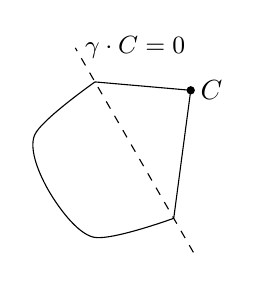
\begin{tikzpicture}[rotate=30]
      \draw [dashed] (0, -1.5) -- (0, 1.5) node [right] {\small$\gamma \cdot C = 0$};
      \draw (0, 1) -- (1, 0.3) node [circ] {} node [right] {$C$} -- (0, -1);
      \draw plot [smooth] coordinates {(0, 1) (-1, 0.8) (-1.2, 0.1) (-1, -0.7) (0, -1)};
    \end{tikzpicture}
  \end{center}
  To the left of the dahsed line is $\overline{\NE(X)}_{C \geq 0}$, which we can say nothing about, and to the right of it is a ``cone'' to $C$, generated by interpolating $C$ with the elements of $\overline{\NE(X)}_{C \geq 0}$.

  Thus, $[C] \in N_1(X)_\R$ is an extremal ray of $\overline{\NE(X)}$. In other words, if
  \[
    \lambda [C] = \mu_1 \gamma_1 + \mu_2 \gamma_2
  \]
  where $\mu_i > 0$ and $\gamma_i \in \overline{\NE(X)}$, then $\gamma_i$ is a multiple of $[C]$.
\end{eg}

%\begin{eg}
%  We continue to think about surfaces. One way to construct surfaces is as follows: Take a smooth projective curve of genus $g$. Let $U$ be a vector bundle on $C$ of rank $2$ and degree $0$. We can then define $X = \P(U) \overset{\pi}{\to} C$, and $X$ is a surface.
%
%  One can show using the localization sequence that
%  \[
%    N^1(X)_\R = \R[F] + \R[\mathcal{O}_{\P(U)}(1)],
%  \]
%  where $F$ is a fiber of $\pi$. We write $\psi$ for $\mathcal{O}_{\P(U)}(1)$. It is clear that $F^2 = 0$, since different fibers don't intersect, and also $F \cdot \psi = 1$, since $\mathcal{O}_{\P(U)}(1)$ restricted to $F$ is just $\mathcal{O}(1)$. We also have $\psi^2 = \deg U = 0$. So the intersection product is given by
%  \[
%    (aF + b\psi)^2 = 2 ab.
%  \]
%  So we find that $\Nef(X)$ is contained in the first first quartile $\R^+ [F] + \R^+ [\psi]$.
%
%  Note that there is a one-to-one correspondence between sections of $\pi$ and splittings
%  \[
%    0 \to L_1 \to V \to L_2 \to 0\tag{$*$}
%  \]
%  where $L_1, L_2$ are line bundles. Since $V$ has degree zero, we always have $\deg L_1 = - \deg L_2$. A section of $\pi$ gives a curve $C \subseteq X$ such that $C \cdot F = 1$. Thus, $C$ is of the form
%  \[
%    [C] = [\xi + aF]
%  \]
%  for some $a$. To determine this $a$, note that $C \in H^0(\mathcal{O}_{\P_C(V)}(1) \otimes L_1^\vee)$. So we have $a = \deg L_2$.
%
%  Then $C^2 = 2a$. Now if $a = \deg (L_2) < 0$, then $[C]$ is an extremal ray of $\overline{\NE(X)}$. Since $F^2 = 0$, we know $[F]$ is the extremal ray, and the Nef cone is the dual, hence has extremal rays $F$ and $-aF + \xi$.
%
%  It follows from this description that $\NE(X) = \overline{\NE(X)}$. If $V$ is semistable, i.e.
%  \[
%    \deg (L_2) \geq 0\text{ in }(*),
%  \]
%  then $\Sym^n V$ are also semistable. % i.e.\ if there is a sujection $\Sym^n V \twoheadrightarrow L$, then $\deg (O) \geq 0$.
%
%  Now a curve $E \subseteq X$ corresponds to sections of $\mathcal{O}_{\P_V(C)} (n) \otimes \pi^*(A)$ for $A$ a line bundle on $C$. Then the globla sections of this correopnd to $H^0(C, \Sym^n V \otimes A)$. If $h^0 \not= 0$, then semi-stability means if $\deg A \geq 0$. So $\overline{\NE(X)} = \R^+ \xi + \R^+ F$.
%
%  Is $\NE(X)$ closed? In other words, is $\R^+ \xi$ spanned by an effective $1$-cycle? If the answer is no, then we see an explicit example that using Kleinmann's criterion, we actually need to use $\overline{\NE(X)}$.
%
%  The answer is actually no in general.
%\end{eg}
%
%\begin{thm}[Hartshorne]
%  If $g(C) \geq 2$, then there exists a semi-stable vector bundle $V$ of degree $0$ over $C$ such that $H^0(\Sym^nV \otimes A) = 0$ for all $A \in \Pic^0(C)$ and all $n \geq 0$.\fakeqed
%\end{thm}
%In fact, this is a generic phenomenon.

In fact, in general, we have
\begin{thm}[Cone theorem]
  Let $X$ be a smooth projective variety over $\C$. Then there exists rational curves $\{C_i\}_{i \in I}$ such that
  \[
    \overline{\NE(X)} = \overline{\NE}_{K_X \geq 0} + \sum_{i \in I} \R^+ [C_i]
  \]
  where $\overline{\NE}_{K_X \geq 0} = \{\gamma \in \overline{\NE(X)} : K_X \cdot \gamma \geq 0\}$. Further, we need at most countably many $C_i$'s, and the accumulation points are all at $K_X^\perp$.
\end{thm}

%\begin{eg}
%  If $X$ is a surface. If $K_X$ is not nef, either we can find a curve $C$ with
%  \begin{enumerate}
%    \item $K_X \cdot C = -1$, where we can blow down the curve;
%    \item $K_X \cdot C = -2$, then $X \to C $ is a $\P^1$-bundle;
%    \item $K_X \cdot C = -3$, where we are $\P^2$.
%  \end{enumerate}
%  If we know a priori that (ii) and (iii) are not the case, then we can keep blowing down until either $K_X$ is nef or (ii) or (iii). Then for some large $m$, we have $|m K_{X_m}| \not= 0$ and base-point free. This then gives a canonical model $Y$ with a map $X_n \to Y$ given by
%  \[
%    \Proj\left(\bigoplus_{m \geq 0} H^0(mK_X)\right) = \Proj \left(\bigoplus_{m \geq 0} H^0 (mK_X)\right).
%  \]
%\end{eg}
%This is generalized to things that are not surfaces. % minimal model program

\subsection{Kodaira dimension}
Let $X$ be a normal projective variety, and $\mathcal{L}$ a line bundle with $|\mathcal{L}| \not= 0$. We then get a rational map
\[
  \varphi_{|\mathcal{L}|}: X \dashrightarrow \P(H^0(\mathcal{L})).
\]

More generally, for each $m > 0$, we can form $\mathcal{L}^{\otimes m}$, and get a rational map $\varphi_{\mathcal{L}^{\otimes m}}$. What can we say about the limiting behaviour as $m \to \infty$?
%
%We can do the same for all $m > 0$ with $\mathcal{L}^{\otimes m}$. What can we say the limiting behaviour of $m \to \infty$? In particular, do the $\varphi_{|\mathcal{L}^{\otimes m}|}$ display eventually the same behaviour? We have a map
%\[
%   \psi: \bigotimes^m H^0(\mathcal{L}) \to H^0(\mathcal{L}^{\otimes m}).
%\]
%Write $V_m$ for the image of $\psi$. We then have a composition
%\[
%  \begin{tikzcd}
%    X \ar[r, dashed, "\varphi_{|\mathcal{L}^{\otimes m}|}"] & \P(H^0(\mathcal{L}^{\otimes m})) \ar[r, "\mathrm{proj}"] & \P(V_m)
%  \end{tikzcd}
%\]
%The composition is then just the $m$th veloromes of $\varphi|_{\mathcal{L}}$. % fix the v-something word.

\begin{thm}[Iitaka]
  Let $X$ be a normal projective variety and $\mathcal{L}$ a line bundle on $X$. Suppose there is an $m$ such that $|\mathcal{L}^{\otimes m}| \not= 0$. Then there exists $X_\infty, Y_\infty$, a map $\psi_\infty: X_\infty \to Y_\infty$ and a birational map $U_\infty: X_\infty \dashrightarrow X$ such that for $K \gg 0$ such that $|\mathcal{L}^{\otimes K}| \not= 0$, we have a commutative diagram
  \[
    \begin{tikzcd}
      X \ar[r, dashed, "\varphi_{|\mathcal{L}^{\otimes k}|}"] & \Im (\varphi_{|\mathcal{L}^{\otimes K}})\\
      X_\infty \ar[u, "U_\infty", dashed] \ar[r, "\psi_\infty"] & Y_\infty \ar[u, dashed]
    \end{tikzcd}
  \]
  where the right-hand map is also birational.
\end{thm}
So birationally, the maps $\psi_K$ stabilize.

\begin{defi}[Kodaira dimension]\index{Kodaira dimension}
  The \emph{Kodaira dimension} of $\mathcal{L}$ is
  \[
    K(X, \mathcal{L}) =
    \begin{cases}
      -\infty & h^0(X, \mathcal{L}^{\otimes m}) = 0\text{ for all }m > 0\\
      \dim (Y_\infty) & \text{otherwise}
    \end{cases}.
  \]
\end{defi}
This is a very fundamental invariant for understanding $\mathcal{L}$. For example, if $K(X, \mathcal{L}) = K \geq 0$, then there exists $C_1, C_2 \in \R_{>0}$ such that
\[
  C_2 m^K \leq h^0(X, \mathcal{L}^{\otimes m}) \leq C_1 m^K
\]
for all $m$. In other words, $h^0(X, \mathcal{L}^{\otimes m}) \sim m^K$.

\printindex
\end{document}
